%%%%%%%%%%%%%%%%%%%%%%%%%%%%%%%%%%%%%%%%%
% Based on the report template by Andrea Hidalgo (mrs.petzl@gmail.com)
%
% Important note:
% Chapter heading images should have a 2:1 width:height ratio,
% e.g. 920px width and 460px height.
%%%%%%%%%%%%%%%%%%%%%%%%%%%%%%%%%%%%%%%%%

%----------------------------------------------------------------------------------------
%	PACKAGES AND OTHER DOCUMENT CONFIGURATIONS
%----------------------------------------------------------------------------------------

% TIP: files with large pictures may have compilation time-out problems on Overleaf. Whenever that happens, switch the preview to Manual, then un-comment the first line below, comment the second line, and compile (refresh preview) once. Once the preview shows without the pictures, revert back to the original documentclass-commenting configuration, and compile again.

%\documentclass[11pt,fleqn,draft]{book} % Default font size and left-justified equations
\documentclass[11pt,fleqn]{book} % Default font size and left-justified equations


 \usepackage[top=3cm,bottom=3cm,left=2.5cm,right=2.5cm,headsep=10pt,a4paper]{geometry} % Page margins



\usepackage[dvipsnames]{xcolor} % Required for specifying colors by name
\definecolor{ocre}{RGB}{52,177,201} % Define the orange color used for highlighting throughout the book

% Font Settings
\usepackage{avant} % Use the Avantgarde font for headings
%\usepackage{times} % Use the Times font for headings
\usepackage{mathptmx} % Use the Adobe Times Roman as the default text font together with math symbols from the Symbol, Chancery and Computer Modern fonts
\usepackage{microtype} % Slightly tweak font spacing for aesthetics
\usepackage[utf8]{inputenc} % Required for including letters with accents
\usepackage[T1]{fontenc} % Use 8-bit encoding that has 256 glyphs
% \usepackage{cite}% citacoes referencias

% BOX style
\usepackage{amsmath} % make box
\usepackage{tcolorbox} % color box
\usepackage{tikz} % include figures in BOX
%\tcbset{every box/.style={{colback=Green!5!white,colframe=Green!75!black} % default setting to connect boxes
\usepackage{geometry}
\usepackage{float}
\usepackage{wrapfig}
\usepackage{lipsum,multicol} % preamble, to break box and align with text
\usepackage{float} % fix de figure in the text
\usepackage{verbatimbox}
\usepackage{caption}

% BOXES styles -all boxes
\newenvironment{mybox}[1]
{\newcounter{mybox}
%\DeclareRobustCommand{\themybox}{\refstepcounter{mybox}\themybox}
% \stepcounter{mybox}%
 \addtocounter{mybox}{1}
 \renewcommand{\themybox}{\arabic{mybox}}
\tcbset{fontupper=\Large,fonttitle=\Large, breakable,colback=Green!5!white,colframe=Green!75!black,title=Box~\themybox\,: #1}
\begin{tcolorbox}}
{\end{tcolorbox}}

% Bibliography
\usepackage[round]{natbib}
%\usepackage[style=alphabetic,sorting=nyt,sortcites=true,autopunct=true,babel=hyphen,hyperref=true,abbreviate=false,backref=true,backend=biber]{biblatex}
%\addbibresource{iis.bib} % BibTeX bibliography file
%\defbibheading{bibempty}{}


%Table-related commands
\usepackage{array}%merge columns
\usepackage{ragged2e} %tamanho das colunas
\usepackage[table]{xcolor}
%\setlength{\arrayrulewidth}{0.2mm}
%\setlength{\tabcolsep}{18pt}
%\renewcommand{\arraystretch}{1.5}
%\newcolumntype{s}{>{\columncolor[HTML]{AAACED}} p{3cm}}
\usepackage{multirow}
\usepackage{longtable}

\usepackage[utf8]{inputenc}
\usepackage{fourier} 

\usepackage{makecell}

\renewcommand\theadalign{bc}
\renewcommand\theadfont{\bfseries}
\renewcommand\theadgape{\Gape[4pt]}
\renewcommand\cellgape{\Gape[4pt]}


% Color scheme: refer to latex_colors.png included in the template's root dir
\newcommand{\titlecolor}{White}
\newcommand{\subtitlecolor}{White}
\newcommand{\subsubtitlecolor}{Green}

\newcommand{\sectioncolor}{ForestGreen}
\newcommand{\subsectioncolor}{Orange}
\newcommand{\subsubsectioncolor}{Green}

\newcommand{\headerfillcolor}{Black}
\newcommand{\headerlinecolor}{ForestGreen}

\newcommand{\headertextcolor}{Black}
\newcommand{\maintextcolor}{Black}


%\newcommand{\squeezeup}{\vspace{-3.5mm}}%to reduce space after figures
\input{structureve} % Insert the commands.tex file which contains the majority of the structure behind the template

%\titleformat{\section}{\Large\bfseries}{\thesection}{1em}{}

% \titleformat*{\section}{\bfseries\sffamily}
% \titleformat*{\subsection}{\bfseries\sffamily}

% Remove page from the bottom of the page
\cfoot{}


\begin{document}

% FONT SIZE
\Large


% Color scheme: refer to latex_colors.png included in the template's root dir



%----------------------------------------------------------------------------------------
%	COVER PAGE
%----------------------------------------------------------------------------------------

\begingroup
\thispagestyle{empty}
%\AddToShipoutPicture*{\put(0,0){\includegraphics{pictureve/capa.png}}} % Cover image 
%\centering
\vspace*{17.3cm}
%
\noindent
% First version 
\fontsize{32}{39}{\color{\titlecolor} \textbf{Impacts from Forest and \\[0.2cm] Landscape Restoration \\[0.2cm] in the  
Brazilian Atlantic \\[0.27cm] Forest   and Amazon }}        
% Second version
% \fontsize{32}{33}{\color{\titlecolor} \textbf{Impacts from Forest {\Huge and} \\[0.2cm] Landscape Restoration \\[0.2cm] {\Huge in the}
% Brazilian Atlantic  Forest \\[0.2cm]   {\Huge and} Amazon }}        

% \par\normalfont\fontsize{33}{33}\sffamily\selectfont
% {\color{\titlecolor} \textbf{Impacts from Forest and Landscape Restoration in the 
% Brazilian Atlantic Forest and Amazon}}\\ 

%\includegraphics[width=.6\textwidth,center]{example-image}
% \begingroup
% \thispagestyle{empty}
% \AddToShipoutPicture*{\put(0,0){\includegraphics[scale=2.25]{pictureve/capa.png}}} % Cover image 
% \centering
% \vspace*{6cm}
% \par\normalfont\fontsize{33}{33}\sffamily\selectfont
% {\color{\titlecolor} \textbf{Unlocking Forest Finance}}\\ 

\vspace{0.8cm}
\noindent
{\LARGE  \color{\subtitlecolor} \sc International Climate Initiative (IKI) 
%INTERNATIONAL CLIMATE INITIATIVE (IKI)
}
%\par  
\endgroup

%----------------------------------------------------------------------------------------
%	DISCLAIMER PAGE
%----------------------------------------------------------------------------------------

\newpage
~\vfill
\thispagestyle{empty}

% List of authors / partners
\noindent \textsc{International Institute for Sustainability}

%\noindent \textsc{WRI}

%\noindent \textsc{Governo Alemao}

%\noindent \textsc{\textcolor{red}{MMA- cf André}}



\vspace{1 cm}

% Funding acknowledgement
\noindent {\it This report is part of the Project entitled "Unlocking economic opportunities to scale FLR".}

\vspace{0.75 cm}

% Current date
\noindent \textit{\today}

%~\vfill
\vspace{2 cm}

% Partner-institutions´ logos
\begin{figure}[!htb]

 \minipage{0.15\textwidth}
\includegraphics[width=4.65 cm]{iislogo.png}
\endminipage\hfill
\minipage{0.5\textwidth}
\includegraphics[width=6.70 cm]{pictureve/Logo-deustch.jpg}
\endminipage\hfill
\end{figure}
% \minipage{0.15\textwidth}
%   \includegraphics[width=\linewidth]{logo_gcp.png}
% \endminipage\hfill

%----------------------------------------------------------------------------------------
%	Equipe
%----------------------------------------------------------------------------------------

\chapterimage{Time.png}

%%%%%%%%%%%%%%%%%%%%%%%%%%%%%%%%%%%%%%%%%%%%%%%%%%%%%%%%%%%%%%
% Equipe
%%%%%%%%%%%%%%%%%%%%%%%%%%%%%%%%%%%%%%%%%%%%%%%%%%%%%%%%%%%%%%


\chapter*{Team} \label{ch:equipe}

 \textbf {\underline{Executive Directors}}\\[0.3cm]
 Bernardo Strassburg \\
 Agnieszka Latawiec 
\\[0.7cm]
\textbf{\underline{Technical Coordination}}\\[0.3cm]
Renato Crouzeilles\\
Veronica Maioli\\
Catarina Jakovac\\
André Junqueira\\

\\[0.7cm]
\noindent{\textbf{\underline{{Execution Team}}}\\[0.3cm]
\begin{tabular}{ll}
\hspace{-0.3cm} Mariela Figueredo ({\em Project Manager})\\

\hspace{-0.3cm} Aline Rodrigues & Ingrid Pena\\

\hspace{-0.3cm} Alvaro Iribarrem & Isabelle Pepe \\

\hspace{-0.3cm} Ana Castro & Katarzyna A Korys\\

\hspace{-0.3cm} Carlos Cordeiro & Lara Monteiro \\

\hspace{-0.3cm} Eduardo Lacerda & Luisa Lemgruber\\

\hspace{-0.3cm} Eric Lino & Maiara Mendes\\

\hspace{-0.3cm} Fernanda Tubenchlak & Viviane Dib\\

\hspace{-0.3cm} Gustavo Malaguti & Yuri de Carvalho\\ 
 

\end{tabular}

   
% \noindent Mariela Figueredo (Projet Manager)

% \noindent Alvaro Iribarrem (Modeling specialist)

% \noindent Carlos Cordeiro (GIS specialist)

% \noindent Eduardo Lacerda (GIS specialist)

% \noindent Eric Lino (GIS specialist)

% \noindent Aline Rodrigues (Research assistant)

% \noindent Fernanda Tubenchlak (Research assistant)

% \noindent Gustavo Malaguti (Research assistant)
 
% \noindent Lara Monteiro (Research assistant)

% \noindent Luisa Lemgruber (Research assistant)

% \noindent Ingrid Pena (Research assistant)

% \noindent Isabelle Pepe (Research assistant)

% \noindent Katarzyna Anna Korys (Research assistant)

% \noindent Maiara Mendes (Research assistant)

% \noindent Viviane Dib (Research assistant)

% \noindent Yuri Carvalho (Trainee)


%----------------------------------------------------------------------------------------
%	Glossario
%----------------------------------------------------------------------------------------

%input{Glossario.tex}


%----------------------------------------------------------------------------------------
%	TABLE OF CONTENTS
%----------------------------------------------------------------------------------------

%\newpage

\chapterimage{contents.png} % Table of contents heading image

\pagestyle{empty} % No headers

\tableofcontents % Print the table of contents itself

%\cleardoublepage % Forces the first chapter to start on an odd page so it's on the right

\pagestyle{fancy} % Print headers again
%----------------------------------------------------------------------------------------
%	EXECUTIVE SUMMARY
%----------------------------------------------------------------------------------------

 

\chapterimage{summary.png} % Chapter heading image

%%%%%%%%%%%%%%%%%%%%%%%%%%%%%%%%%%%%%%%%%%%%%%%%%%%%%%%%%%%%%%
% Executive_summary
%%%%%%%%%%%%%%%%%%%%%%%%%%%%%%%%%%%%%%%%%%%%%%%%%%%%%%%%%%%%%%

\chapter*{Executive summary}\label{ch:summary}

Forest  and  Landscape  Restoration  (FLR) is  a  process of regaining ecological functionality and enhancing human well-being in previously forested landscapes. Yet, its outcomes for biodiversity, climate change mitigation, water and socio-economic dimensions remains scarce. The present report provides a review of FLR impacts on different aspects of biodiversity (section \ref{ch:biodiv}), climate change mitigation (section \ref{ch:carbon}), water (section \ref{ch:water}), and socioeconomic dimensions (section \ref{ch:socio}), and introduce on-going methodologies for developing spatial explicit models for supporting decision making in two of Brazilian biomes with the highest demands for large-scale restoration (Atlantic Forest and Amazon). It also produce preliminary key guidelines for decision makers and restoration practitioners on FLR and its impacts (section \ref{ch:recom}).

FLR outcomes for biodiversity depend on processes related with the (re) colonization, supplementation and maintenance of wildlife species and popu-lations in restored systems and surrounding landscapes. In section 2, we quantify these processes in terms of biodiversity restoration, species connectivity and species extinction risk. Therefore, we conducted a: (i) literature review on the impacts of different restoration methods on biodiversity for all Brazilian biomes, (ii) quatitative comparisons for biodiversity between nega-tive reference (e.g. agriculture and pasturelands), simple and biodiverse agroforestry systems with original reference systems (e.g. less disturbed or old-growth forests) for the Atlantic Forest, (iii) spatial analysis to illustrate the importance of incorporating landscape connectivity in FLR planning for biodiversity recovery in the Atlantic Forest, and (iv) spatial analysis to mapping the probability of extinction for endemic Atlantic Forest species as a function of the marginal contribution of each hectare restored to reducing species’ extinction probability.

FLR can play an important role in mitigating climate change as Tropical forest restoration can sequester large amounts of carbon from the atmosphere into the above and below-ground biomass and into the soil. In the section 3, we conducted a: (i) systematic literature review to understand how restoration initiatives in the Atlantic Forest have accounted for soil indicators in their planning and management decisions, (ii) literature review  on the impacts of different restoration methods on carbon stock for all Brazilian biomes, and (iii) spatial analysis to map the potential carbon sequestration by FLR in Brazil.

FLR has emerged as a feasible solution for water regulation and purification as forests can perform eco-hydrological functions, as regulation of water flow and maintenance of water quality. In the section 4, we study the FLR impacts on water quality and quantity by: (i) conducting a spatial analysis to investigate soil loss and sediment exportation to water under different FLR scenarios in the Atlantic Forest, (ii) conducting an international workshop to better understand the relationships between FLR and water, (iii) proposing a new approach to prioritize areas for FLR based on water quality improvement and a methodology to access the impact of large-scale restoration scenarios on Amazon and Atlantic Forest precipitation patterns.

The success or failure of a FLR project depends not only ecological, but also on socioeconomic factors as forests and trees contribute in multiple ways through a variety of ecosystem services to alleviate poverty, reduce food insecurity and support sustainable livelihoods. In the section 5, we conducted a: (i) systematic review consolidating the existing literature regarding restoration, socioeconomic benefits and ecosystem services provision, and (ii) propose two strategies to include socioeconomic aspects into spatial restoration prioritization in the Amazon and Atlantic Forest biomes. 

Finally, this report also provides 11 key preliminary recommendations for guiding decision makers and restoration practitioners on FLR and its impacts on the topics discussed above. These recommendations are critical to allow the sustainability and replicability of restoration projects. This report aim to help unlock the flow of financial investments needed to implement the ambitious Brazilian restoration targets and commitments.



%----------------------------------------------------------------------------------------
%	CHAPTER:  Introduction
%----------------------------------------------------------------------------------------
\chapterimage{FLR.jpg}



%%%%%%%%%%%%%%%%%%%%%%%%%%%%%%%%%%%%%%%%%%%%%%%%%%%%%%%%%%%%%%%%%%%%%%%%%%%%%%%%%%%%%%%%%%%%%%%%
% Introduction
%%%%%%%%%%%%%%%%%%%%%%%%%%%%%%%%%%%%%%%%%%%%%%%%%%%%%%%%%%%%%%%%%%%%%%%%%%%%%%%%%%%%%%%%%%%%%%%

\chapter{Forest Landscape Restoration in Brazil} \label{ch:intro}

The  high levels of deforestation and forest degradation, combined with the serious threats from climate change, have stimulated the international community to set international and country-led efforts aiming to boost Forest and Landscape Restoration worldwide (Box \ref{Box1}). The Aichi Targets 14 and 15 of the United Nations Convention on Biological Diversity, for example, aim to restore at least 15\% of degraded ecosystems, the Bonn Challenge and the New York Declaration on Forests of the United Nations 
 Climate Summit seeks to restore 150 and 350 M ha of degraded and deforested lands by 2020 and 2030, respectively \citep{Chazdon2017d}. Other remarkable efforts are the Initiative 20x20 in Latin America and the AFR100  in Africa, which seeks to restore 20 and 100 M ha of deforested and  degraded lands by 2020 and 2030, respectively \citep{Chazdon2017b}.
 
%%%%%%%
%%%%% BOX 1- FLR %%%%%%%%%%%%%%%%%%%%%


\begin{wrapfigure}[9]{r}{7.4cm}
\begin{mybox}{Defining  Forest and Landscape Restoration (FLR)}
\label{Box1}
FLR is a process of regaining ecological functionality and enhancing human well-being in previously forested landscapes (IUCN 2018).
\end{mybox}
\end{wrapfigure}
%
In the Brazilian context, two main instruments foster and regulate FLR: the Native Vegetation Protection Law (NVPL; Federal Law No 12,651/2012) and the National Plan for Native Vegetation Recovery (PLANAVEG). The NVPL is the main environmental law that protects the use of native vegetation in rural landholdings, replacing the previous Forest Code \citep{Soares-filho2014}. After a long period of discussion and debates, the new law established for the first time a governance structure and enforcement mechanisms for promoting the restoration of native ecosystems and the conservation of native ecosystems in rural landscapes. \\
\indent In a context of integrated landscape management, the NVPL determine that rural properties must conserve native forest, or restore them when necessary, in a portion of their land which depends on the Biome and property size (named Legal Reserve; for example, 20\% and 80\% in the Brazilian Atlantic Forest and Amazon biomes, respectively), and in areas with special ecologi-cal interest such as riparian forests, water springs, hilltops and slopes over 45$^{o}$ degrees (named Permanent Preserved Areas). Under the NVPL, agricultural credits will be restricted only to farmers that comply with the environmental law, as a way to enforce and guarantee restoration and conservation actions. The PLANAVEG is a top-down process conducted by the Brazilian Environmental Ministry, which joined effort with academia, private sector, NGOs, and state governments since 2013, to motivate and create the enabling conditions and incentives for rural landowners to restore at least 12.5 M ha of degraded and deforested lands by 2030 in Brazil \citep{Brasil2017}. This target is aligned with the estimated environmental debits enforced by the NVPL and the Brazil’s national and international commitments to the Aichi, Nationally Determined Contribution, the Bonn Challenge and the Initiative 20x20 targets. Therefore, Brazilian restoration practitioners, researchers, stakeholders and decision-makers face a key implementation challenge to reach the ambitious restoration targets set for the next decades.\\
%
\indent The Amazon and Atlantic Forest are the two Brazilian biomes with the highest demand for restoration of native vegetation, with each biome holding approximately 5 M ha of deforested and degraded land to be restored by law \citep{Brasil2017}. The Amazon and Atlantic Forest biomes lost, respectively, almost 18\% and 68\% of their original vegetation \citep{MAPBIOMAS2018Collection2000-2016}. Deforestation has been mainly driven by the expansion of agriculture and pasturelands, having important impacts on species conservation and on the emission of greenhouse gases to the atmosphere. The region embraced by the Atlantic Forest biome was responsible in 2017 for 24\% of the Brazilian greenhouse gas emissions, which were mainly produced by the agriculture and energy sectors \citep{SEEG2018TabelaDados}. The Amazonian region contributes to 33\% of Brazilian emissions and those are mainly produced by agricultural activities and land-use change \citep{SEEG2018TabelaDados}. Land use change also leads to the reduction of habitat for native species threatening biodiversity conservation. It is currently estimated that in the Amazon 183 fauna species are endangered (being 122 endemics), while in the Atlantic Forest this number reaches 589 fauna species (428 endemic). These biomes also play important roles in the national economy, given that it shelters 63\% of the Brazilian population (ca. 10\% and 53\% in the Amazon and Atlantic Forest) and almost 61.4\% of the Brazilian GDP (7.1\% and 54.3\% in the Amazon and Atlantic Forest, respectively) \citep{20182018Contas2018}. 

Although scaling up FLR is difficult, lengthy, expensive and budget-limited \citep{Crouzeilles2016}, it can offset some of the profound negative impacts of human development on ecosystems through the delivery of multiple bene-fits such as habitats for biodiversity, climate change mitigation, clean water provision, and sustainable livelihoods for people \citep{Chazdon2016c, Holl2017}. Consensus exists that each dollar invested in restoration needs to be spent in the most ecologically and economically efficient way \cite{Ding2017, Verdone2017}. 

The present report provides a review of FLR impacts on different aspects of biodiversity (section \ref{ch:biodiv}), climate change mitigation (section \ref{ch:carbon}), water (section \ref{ch:water}), and socioeconomic dimensions (section \ref{ch:socio}), and and introduce on-going methodologies for developing spatial explicit models for supporting decision making in two of Brazilian biomes with the highest demands for large-scale restoration (Atlantic Forest and Amazon). It also produce preliminary key guidelines for decision makers and restoration practitioners on FLR and its impacts (section \ref{ch:recom}). This report do not aim to extensively review all aspects from FLR impacts, but to better understand and spatially map key FLR impacts, which may help unlock the flow of financial investments needed to implement the ambitious Brazilian restoration targets and commitments.



%----------------------------------------------------------------------------------------
%	CHAPTER 1: Biodiversity
%----------------------------------------------------------------------------------------

\chapterimage{biodiversity.jpg} % Chapter heading image


%%%%%%%%%%%%%%%%%%%%%%%%%%%%%%%%%%%%%%%%%%%%%%%%%%%%%%%%%%%%%%%%%%%%%%%%%%%%%%%%%%%%%%%%%%%%%%%%
% Biodiversity
%%%%%%%%%%%%%%%%%%%%%%%%%%%%%%%%%%%%%%%%%%%%%%%%%%%%%%%%%%%%%%%%%%%%%%%%%%%%%%%%%%%%%%%%%%%%%%%%


\chapter{FLR impacts on biodiversity\label{ch:biodiv}} 

Due to the severe degradation of ecosystems by human activities (e.g. land clearing, fragmentation), the persistence and representation of several species currently depend not only on habitat protection, but also on habitat restoration \citep{Crouzeilles2015}. Restored ecosystems should meet two  conservation objectives for biodiversity: representativeness and persistence \citep{NossReedNielsenScottVance-Borland1982}. The first objective claims that restored ecosystems should be representative of the variety of populations, species and ecosystem functions within each region, while the second aims to guarantee the long-term persistence of these elements in the landscape \citep{Margules2000}. Both objectives depend on processes related with the (re)coloniza-tion, supplementation and maintenance of wildlife species and populations in restored systems and surrounding landscapes \citep{Helmer2008, Crk2009, Crouzeilles2016a}. Here we quantified these processes in terms of biodiversity restoration, species connectivity and species extinction risk. 
%
%-----------------------------------------------------------------------------------------------
\section{\Large Biodiversity restoration}\label{sec:bio-recov}
\subsection{\large Biodiversity restoration using different restoration methods} \label{subsec:bio-revisão}
%
There is an increasing global understanding of biodiversity restoration patterns within two key types of restoration methods: active restoration and natural regeneration (also referred as passive restoration) (e.g. Crouzeilles \cite{Crouzeilles2017a}; Box\ref{Box2}), but we know little on how it applies to specific biomes. Aiming to understand how restoration has impacted biodiversity conservation and climate change mitigation (section \ref{ch:carbon}), we have conducted a literature review on studies on the impacts of different restoration methods on biodiversity and carbon stocks in Brazil. We conducted a systematic literature review searching the databases Scopus, Web of Science, Science Direct, Scielo and Periódicos Capes for published articles, using Boolean searches with the word strings Carbon* OR Biomass OR Biodiversity OR Diversity OR Richness AND restorat* OR natural regeneration OR succession OR Agroforest* in the abstract, title or keywords. We repeated the search in English and in Portuguese. During each search we selected relevant articles based on the abstract and keywords, totaling 202 articles that were included in our literature database using the Mendeley software. \\
\indent Intending to perform a quantitative comparisons (meta-analysis) on how different restoration methods affects biodiversity and carbon stocks (section \ref{ch:carbon}), we have further selected articles according to the following criteria: (i) must provide data on a restoration area (active or passive restoration, agroforest system or silviculture); (ii) must have an original (e.g. a mature or old-growth forest) or negative reference area (e.g. a degraded area or pasture or agricultural land); (iii) must have measured biodiversity and/or carbon and/or biomass stocks in the soil, above and/or belowground components. Such selection has eliminated 92 studies that were out of scope (41 articles, 44\%), did not have a reference ecosystem (36 articles, 39\%), lacked basic information (11, 12\%), or were based on the same data used in another article already included (4, 4\%). We have then retained 110 articles, from which we have already extracted the relevant information to perform the meta-analysis. We extracted information on 44 indicators including location, restoration method, species used, biome, vegetation type, previous land use history, restoration age, pre and post planting management, sample size and mean and variance values for biodiversity and/or carbon and/or biomass metrics from any compartment. Many articles provide poor description on their experimental design and/or do not provide mean and standard deviation values in tables, so when necessary we extracted data from graphs using an image tool (https://automeris.io/WebPlotDigitizer/). We then calculated the standardized mean difference (response ratio) between the biodiversity or carbon values from each restored area and the reference ecosystems (being an original or negative reference). The compiled dataset already been checked and standardized and is ready for the next step of performing the statistical analyses. \\
\indent Results show that the knowledge on ecological restoration in Brazil is concentrated on forest biomes, being mainly based on the Atlantic forest (63\% of the compiled studies, 69 studies), followed by the Amazon (26\%, 29 studies) (Figure \ref{fig:Bio-Cata-1} A). The restoration method of passive restoration was the most studied in both forest biomes (Figure \ref{fig:Bio-Cata-1} C) probably due to the longest history of studies on secondary forest succession than on active restoration (Figure \ref{fig:Bio-Cata-1} B). Most studies compared the areas under restoration with an original reference and only a few had a negative reference (Figure \ref{fig:Bio-Cata-1} D).  
%
%%%%%% FIgura CATA 1 A-D %%%%%%%% 
\begin{figure}[H]
\includegraphics[width=1.0\linewidth]{pictureve/Bio-Cata-1.pdf}
\caption{(A) Proportion of the compiled studies in each Brazilian biome (AF-Atlantic forest, AM-Amazon, CAA-Caatinga, CE-Cerrado, PAM-Pampa, TRS-Transition between Cerrado and Atlantic Forest or Amazon); (B) Number of studies on the different restoration methods (Passive, Active, Agroforestry, Silviculture) over time; (C) Number of selected studies including each restoration technique in the Atlantic Forest and Amazon; (D) Number of selected studies including a positive or negative reference (some studies had both).}
\label{fig:Bio-Cata-1}
\end{figure}
%

\newpage
Among the 98 studies done in the forest biomes, 79 included some type of biodiversity measure, being 49 and 22 in the Atlantic Forest and Amazon, respectively (Figure \ref{fig:Bio-Cata-2}). As one study may have included more than one biome, the total number of studies available for our meta-analysis is 66 and 28 for the Atlantic Forest and Amazon, respectively. Most selected studies focused on animals followed by plants and soil biology (Figure \ref{fig:Bio-Cata-2}). Although the higher amount of studies on animals than on plants seems unexpected, other meta-analysis found the same pattern in a global scale (e.g. Crouzeilles \citep{Crouzeilles2017a}). Species richness was the most used biodiversity measure (35 and 16 in the Atlantic Forest and Amazon, respectively), while species composition (similarity between restored and natural ecosystems) was the least used metric, only present in 13 studies (8 and 5 in the Atlantic Forest and Amazon).

%
%%%%%% FIgura CATA 2 %%%%%%%%
\begin{figure}[H]
\includegraphics[width=1.0\linewidth]{pictureve/Bio-Cata-2.pdf}
\caption{Number of studies that analyzed the effects of restoration on the biodiversity (A) and abundance (B) in the Brazilian Atlantic Forest and Amazon biomes, and the proportion of studies on animals (ANIM), plants (PLANT), animal-plant together and soil fauna (SOIL-BIOL).}
\label{fig:Bio-Cata-2}
\end{figure}

\newpage
%
%%%% Box tipos de restauracao
\begin{center}
\begin{mybox}{Definitions of actively and passively restored systems, simplified and biodiverse agroforestry systems, degraded and reference systems}
\label{Box2}
{\bf Negative reference:} Agricultural monoculture plantations and monoculture planted forests or pastures, that is, conventional production systems \citep{Crouzeilles2016a}.
%
{\bf Restored systems:} Selectively logged forests or forests in their initial or secondary stage of succession, that is, areas that regenerated after complete or partial clearance \citep{Crouzeilles2016a}. 
    {\bf Passive restoration (or natural regeneration) systems:} Forest regrowth following land abandonment, selective logging or assisted recovery of native tree species through human interventions, such as fencing, to control livestock grazing, weed control, and fire protection \citep{Shono2007, Zahawi2014, Crouzeilles2017a}.
    {\bf Active restoration systems:} Manipulating disturbance regimes through the use of thinning and burning, the establishment of nursery-grown seedlings, direct seeding, or plantations of tree species \citep{Shono2007, Zahawi2014, Crouzeilles2017a}.
%
{\bf Original reference:} Old-growth or less-disturbed forests \citep{Crouzeilles2016a}
%
{\bf Agroforestry systems:} Land management practice where trees, shrubs, agricultural crops, and animals are used simultaneously or sequentially to produce a large range of products such as timber, fiber, fruits, nuts, annual crops, medicinal plants, and oils (OTS/CATIE, 1986, \cite{May2008} . Simple and biodiverse agroforestry systems were classified according to well-established criteria related to the vegetation structure (density, number of layers, and management dynamics), cultivated species richness, and complexity of interactions over time and space \citep{Schroth2004, Steenbock2003, MiccolisAndrewPeneireiroFabianaMongeliMarquesHenriqueRodriguesVieiraDanielLuisMasciaArco-VerdeMarceloFrancioHoffmannMauricioRigonRehderTatianaPereira2016}.
    {\bf Simple agroforestry systems:} Less than five species; up to three layers (often dominant, intermediate, and live coverage); may or may not use native species, and crops are usually planted in alley cropping or rows; and not based on the local ecosystem and ecological succession.
    {\bf Biodiverse agroforestry systems:} Five or more species; more than three layers (generally divided into short, medium, tall, and emergent); based on local ecosystems, which use indigenous local species and exotic species that are similar in ecological function; and uses the local ecological succession throughout the years as a principle, associated with management dynamics and production staggered over time  \cite{Santos2019}.
\end{mybox}
\end{center}

\newpage
%%%%%%%%%%%%%%%%%%%%%%%%%%%%%%%%%
\subsection{\large Biodiversity restoration in agroforestry systems} \label{subsec:bio-recovery-SAF} 

Few studies have quantified the capacity of agroforestry systems to conserve biodiversity. Agroforestry systems have been recommended as a cost-effective strategy that integrates production and biodiversity conservation, and as a restoration method. Under the NVPL, restoration with agroforestry systems is allowed in Legal Reserves and in Permanent Preserved Areas inside small rural properties (over 4 fiscal modulates). There are, however, different types of agroforestry systems \citep{ MiccolisAndrewPeneireiroFabianaMongeliMarquesHenriqueRodriguesVieiraDanielLuisMasciaArco-VerdeMarceloFrancioHoffmannMauricioRigonRehderTatianaPereira2016} which may contribute differently to biodiversity conservation and to ecosystem restoration. \\
\indent We compared values of different ecological metrics for biodiversity (species richness, abundance, diversity and/or similarity) within simplified and biodiverse agroforestry systems, negative reference systems and original reference systems in the Atlantic Forest \citep{Santos2019}. Values of biodiversity recovery were always lower in agroforestry and degraded systems compared to original reference systems (Figure \ref{fig:Bio-Renatinho-1}). Nonetheless, biodiversity recovery was 15\% and 45\% higher in biodiverse agroforestry systems than in simplified agroforestry systems and negative reference systems, respectively. Simplified agroforestry systems had higher values of biodiversity recovery (30\%) than degraded systems. \\
\indent Our results show that agroforestry systems do not result in similar values of biodiversity to those found in old-growth and less-disturbed forests (i.e. full recovery), corroborating the idea that primary forests are indeed irreplaceable for the maintenance of biodiversity \citep{Gibson2011, Crouzeilles2016a}. Agroforestry systems, however, hold significantly higher levels of biodiversity restoration than simplified monocultures, indicating the potential to complement biodiversity conservation and restoration in FLR initiatives. We also found that the type of agroforestry system is critical to determine biodiversity restoration, with biodiverse agroforestry systems recoverying higher levels than simplified agroforestry systems. Combined, these results indicate that biodiverse agroforestry systems may, over long periods of ecological succession, promote the restoration of biodiversity in rural landscapes and should be considered as an alternative restoration method to restore degraded lands in human-modified landscapes that can reconcile sustainable production and biodiversity conservation. 

\newpage
%%%%%% FIgura Bio-Renatinho 1 %%%%%%%%
\begin{figure}[H]
\includegraphics[width=1.0\linewidth]{pictureve/Bio-Renatinho-1.pdf}
\caption{Values of biodiversity recovery for negative reference systems, simple and biodiverse agroforestry systems compared to original reference systems in the Brazilian Atlantic Forest. Negative values (measured as median effect size) means that biodiversity recovery in restored/agroforestry/negative reference systems did not reach a benchmark state yet when compared to original reference systems. The opposite holds for positive values: values of biodiversity in restored/agroforestry/negative reference systems surpasses those found in reference systems. Values around zero are the desired outcome of restoration: when restored/agroforestry/negative reference systems have reached a benchmark level. Dashed lines indicate no significant difference with reference systems. n = sample size, site = number of study landscapes. The box plots show the mean effect size, and the variation of the first and third quartile of resampled response ratios. Notches (triangles) in the boxes represent 95\% confidence intervals and non-overlapping notches between boxes imply a significant difference \citep{Crouzeilles2016a}.}
\label{fig:Bio-Renatinho-1}
\end{figure}


%-----------------------------------------------------------------------------------------------

\section{\Large Landscape connectivity }\label{sec:bio-connect}

In order to allow for effective biodiversity recovery in restored and agroforestry systems, native and restored ecosystems must be connected within landscapes \citep{Crouzeilles2014, Crouzeilles2015}. Landscape connectivity is the degree to which the landscape facilitates or impedes species movements among habitat patches. %(Tayler et al. 1993) Nao estava nas referencias!. 
Landscape connectivity minimizes the effects of habitat loss and fragmentation on biodiversity and improves gene flow, wildlife dispersal, population viability and ecosystem services \citep{Lindenmayer2006, Galpern2011}. The effectiveness of landscape connectivity for biodiversity depends on habitat quality, amount and configuration of the habitat within a landscape, and species dispersal ability. Connectivity, therefore, varies among species in the same landscape, and for the same species among landscapes \citep{CROUZEILLES2013}. 

We used a case study in the surroundings of the Reserva Biológica do Tinguá (State of Rio de Janeiro, Atlantic Forest) to illustrate the importance of landscape connectivity in previously forested regions and of landscape planning for biodiversity recovery (Niemeyer et al. \textit{submited}). According to the NVPL, rural landowners must protect a certain amount of native vegetation in their properties and restore their environmental debts, if they exist, within a specific time-frame. Here we evaluated how landscape connectivity can be improved using two strategies of allocation of restoration in the landscape (maximizing landscape connectivity and random restoration) for three simulated species with different dispersal abilities (10, 700 and 3000m) within three landscapes with different amounts of forest cover (~10, 30 and 50) across the time-frame available for landowner to restore their lands.
	
As expected, the strategy that yielded the greatest improvement in landscape connectivity was "maximizing landscape connectivity", for all species and all landscapes. At the landscape with 13\% forest cover, an increase of 8\% in forest cover after restoration incremented landscape connectivity between 18-148\% (random restoration) and 77-160\% (maximizing landscape connectivity). At the landscape with 24\% forest cover, an increase of 6\% in forest cover after restoration incremented landscape connectivity between 13-47\% (random restoration) and 60-120\% (maximizing landscape connectivity). At the landscape with 44\% of forest cover, an increase of 4\% in forest cover after restoration incremented landscape connectivity between 9-14\% (random restoration) and 17-27\% (maximizing landscape connectivity). Such patterns are a consequence of how restored systems were allocated in the landscape: when maximizing landscape connectivity there was an increase in enlargement and connection among existing habitat patches, while the strategy targeting random restoration resulted in numerous small isolated forest remnants in the landscapes (Figure \ref{fig:Bio-Renatinho-2}).  \\

\newpage

%%%%%% FIgura Bio-Renatinho 2 %%%%%%%% FALTA ALINHAR!!
\begin{figure}[H]
\includegraphics[width=1.0\linewidth]{pictureve/Bio-Renatinho-2.pdf}
\caption{Simulated restored areas based on the strategies targeting random restoration and maximizing landscape connectivity with landscapes with different amounts of forest cover: low (10\%), medium (30\%) and high (50\%). Green: current forest cover, Yellow: restorable areas (i.e. agriculture and pastureland), Red: restored forest cover after 20 years; and Blank: non-restorable areas (i.e. urban areas, rivers and roads). }
\label{fig:Bio-Renatinho-2}
\end{figure}

We reveal three main findings: i) restoration strategies that target for landscape connectivity can accelerate and anticipate biodiversity benefits of restoration initiatives, even when restoration is limited by spatial constrains (e.g. as specified by the NVPL); ii) the benefit of each restoration strategy will depend on both the amount of forest cover in the landscape  and the species dispersal ability; and iii) spatial planning increases effectiveness of restoration initiatives and their outcomes (e.g. biodiversity recovery). \\



%-----------------------------------------------------------------------------------------------


\section{\Large Extinction risk }\label{sec:bio-extinct}

Analyses that account for the probability of avoided extinctions can be a useful tool for subsidizing conservation and restoration policies and practices. To evaluate the effectiveness of a conservation intervention, it is desirable to consider whether the interventions are being able to avoid loss of ecosystems, species or any other valued aspects of the natural environment \citep{Pressey2015}. Most conservation interventions are usually placed in areas where they have least potential for making a difference in species persistence, such as areas suffering from low human pressures \citep{Andam2008}. Differently, landscape restoration initiatives are preferably placed in areas where it can yield the highest impacts on species conservation by, for example, reducing the probability of extinction of a species through restoration of landscapes within the species potential distribution \citep{Thomas2004, Strassburg0StrategicCosts}. In the FLR context, therefore, high-valued areas are those with the potential for delivering the highest number of avoided extinctions across multiple taxonomic groups. 
	
Here we measured the probability of extinction for endemic Atlantic Forest species as a function of the marginal contribution of each hectare restored to reducing species’ extinction probability \cite{Strassburg0StrategicCosts}. In this approach, the value of restoring additional habitat for a species diminishes as the total area of habitat increases. For example, if existing habitat area is small there is a large benefit to increasing that area through restoration, but as the area of habitat restored increases there is a diminishing benefit for the addition of more habitat area restored. We used the potential species distribution instead of the current species distribution because restoration would expand available habitat area for the species. This is different from the usual approach in conservation prioritization where the aim is to conserve current habitats by using species’ distribution that falls within native vegetation.

We generated potential species occurrence models for 2,392 species of plants (n = 2,046), birds (n = 223) and amphibians (n = 123) native to the Brazilian Atlantic Forest (Figure \ref{fig:Bio-Extinct-1}). The overlay of the potential distribution maps for all taxonomic groups shows that the highest species’ richness are found along the Brazilian coast, specially within the States of Rio de Janeiro, São Paulo, Paraná, Santa Catarina and Rio Grande do Sul, and also extending to inner regions of Minas Gerais in the transition to the Cerrado biome. From this set of species, 33\% (n = 785) are endemic to the biome and were used to calculate the avoided extinction risk (Figure \ref{fig:Bio-Extinct-2}).  \\
 
 \newpage
 %%%%%% FIgura Bio-Extinct-1 %%%%%%%% 
\begin{figure}[H]
\includegraphics[width=1.0\linewidth]{pictureve/Bio-Extinct-1.pdf}
\caption{Potential species richness distribution across the Brazilian Atlantic Forest for (a) woody plants, (b) birds and (c) amphibians. The darker the colour the higher the species richness in the planning unit.}
\label{fig:Bio-Extinct-1}
\end{figure}
 
 %Figure 5. \textcolor{blue}{FIGURA-BIODIV-EXTINC-1.} Potential species richness distribution across the Brazilian Atlantic Forest for (a) woody plants, (b) birds and (c) amphibians. The darker the colour the higher the species richness in the planning unit. \\
 

We aggregated the avoided extinction risk at each planning unit across all endemic species, thereby generating a FLR biodiversity-benefits surface. Our results show that the highest number of avoided extinctions of endemic species (Figure \ref{fig:Bio-Extinct-2}) coincides with the areas holding the highest species richness in the biome (Figure \ref{fig:Bio-Extinct-1}). Despite less biodiverse, the northeastern Brazil would also greatly benefit from restoration, especially avoiding the extinction of bird and amphibian species. Restoration in the southeastern region of the State of Bahia, for example, would importantly reduce species extinction risk as it is considered a global hotspot of biodiversity, holding one of the highest levels of plant species richness in the world \citep{Thomas1998}, and being an important center of endemism for amphibians. FLR in these areas, which have been highly deforested in the past, would yield the highest benefits for biodiversity conservation and therefore should be prioritized when planning restoration aiming to conserve biodiversity.  \\

\newpage
 %%%%%% FIgura Bio-Extinct-2 %%%%%%%% 
\begin{figure}[H]
\includegraphics[width=1.0\linewidth]{pictureve/Bio-Extinct-2.pdf}
\caption{Surface of biodiversity conservation benefits from restoration for amphibians, birds, plants and all species combined. The benefits for biodiversity conservation was measured in terms of avoided extinctions per hectare, and the maps show these benefits for (a) woody plants, (b) birds, (c) amphibians and (d) for all species combined. Importantly, these benefits are shown here for the starting situation. As restoration occurs such pattern will change.}
\label{fig:Bio-Extinct-2}
\end{figure}

%Figure 6.\textcolor{blue}{FIGURA-BIODIV-EXTINC-2.} Surface of biodiversity conservation benefits from restoration for amphibians, birds, plants and all species combined. The benefits for biodiversity conservation was measured in terms of avoided extinctions per hectare, and the maps show these benefits for (a) woody plants, (b) birds, (c) amphibians and (d) for all species combined. Importantly, these benefits are shown here for the starting situation. As restoration occurs such pattern will change.\\








%----------------------------------------------------------------------------------------
%	CHAPTER 2: Carbono
%----------------------------------------------------------------------------------------

\chapterimage{carbon.jpg} % Chapter heading image



%%%%%%%%%%%%%%%%%%%%%%%%%%%%%%%%%%%%%%%%%%%%%%%%%%%%%%%%%%%%%%%%%%%%%%%%%%%%%%%%%%%%%%%%%%%%%%%%
% Carbon
%%%%%%%%%%%%%%%%%%%%%%%%%%%%%%%%%%%%%%%%%%%%%%%%%%%%%%%%%%%%%%%%%%%%%%%%%%%%%%%%%%%%%%%%%%%%%%%%

\chapter{FLR impacts on climate change mitigation} \label{ch:carbon}


Current net carbon emissions due to tropical deforestation and degradation are estimated to contribute to 8-15 \% (approx. 1.1 GtC) of the total global anthropogenic carbon emissions \citep{Houghton2015ACO2, Brinck2017HighCycle}. Deforestation contributes to CO2 emissions by burning the vegetation biomass and releasing carbon from soils \citep{Wang2016DynamicsChina}. Concerns regarding global climate change have motivated policymakers from many countries to implement regulations and policies aiming to minimize national emissions of carbon dioxide \citep{Stavins1997PolicyProblem, Clarkson2015TheScheme}. Historically, efforts have been directed mainly to preventing deforestation and degradation of tropical forests, but FLR can play an important role in mitigating climate change \citep{Chazdon2016c,Locatelli2015TropicalCarbon}. 

Tropical forest restoration can sequester large amounts of carbon from the atmosphere into the above and below-ground biomass (AGB) and into the soil \citep{Silver2000TheLands, Lal2004SoilSecurity, Cunningham2015BalancingRegions}. Neotropical secondary forests, for example, accumulate biomass at a rate 11\% higher than mature forests \citep{Poorter2016}. If all secondary forest currently occurring in the Neotropics is allowed to grow, it can potentially sequester a total of 31.09 Pg CO2 in the next 40 years, which is equivalent to carbon emissions from fossil fuel use and industrial processes in all of Latin America and the Caribbean from 1993 to 2014 \citep{Chazdon2016c}. Another study estimates that restoring 500 million hectares of tropical forests could sequester approximately 1 PgC yr−1 \citep{Houghton2015ACO2}. Although most studies focus on carbon sequestration by the above-ground biomass, vegetation regrowth dynamics and associated biomass decomposition increase organic carbon concentration in the soil forming a stable carbon storage \citep{Xu2018EffectsChina}. 

	Studies have shown that forest restoration can increase C stocks in the soil through the addition of organic carbon from the decomposition of trunks, litter and roots (e.g. \citep{Macedo2008ChangesTrees, RodriguesNogueiraJr.2011SoilSpecies, Xu2018EffectsChina}. Soils can potentially accumulate carbon at a rate of 1.30 Mg ha-1 yr-1 during the first 20 years of forest establishment and at a rate of 0.20 Mg ha-1 yr-1 in the subsequent 80 years \citep{Silver2000TheLands}. Estimates on the potential C sequestration by world soils vary widely, ranging from 0.4 GtC yr -1 to 1.2 GtC yr-1 \citep{Sauerbeck2001CO2emissionsLimitations, Lal2004SoilSecurity}. Such uncertainty is partly related to the fact that the dynamics of carbon cycling in the soil during forest regrowth, particularly in the tropics, is still poorly understood \citep{Ritchie2014PlantGrassland, Wang2016DynamicsChina, Xu2018EffectsChina}. Additionally, past land-use history, restoration age and restoration method (active, natural regeneration or agroforestry systems) are important factors determining the rates of biomass and soil carbon accumulation during tropical forest regeneration. Therefore, there is a need to investigate how efficient different restoration methods can be in different landscape contexts. 


%---------------------------------------------------------------------------------------------
\section{\Large Soil quality indicators for FLR in the Atlantic Forest}  \label{sec:car-air}

Consideration of soil quality indicators is crucial for planning the management and restoration of ecosystems. We conducted a systematic literature review to understand how restoration initiatives in the Atlantic Forest have accounted for soil indicators in their planning and management decisions \citep{Mendes2018}. From the 152 retrieved studies, only 41\% (62) reported any soil data. Among those, only 40\% of the retrieved studies included information on soil conditions before the restoration took place (project baseline) or from reference sites. Out of the studies that had reference sites (N =25), the most cited soil indicators were Phosphorus and pH (56\%, N=14) followed by carbon (52\%; N=13), potassium (48\%; N =12), nitrogen (44\%; N =11), aluminium (31\%; N =8), edaphic fauna (20\%;N =5), CEC (16\%; N =4), and iron (12\%; N =3). It was surprising that soil organic matter, a fundamental indicator for ecosystem services such as carbon sequestration, was rarely evaluated. 

The results of this work demonstrate a soil data gap within the restoration projects in the Brazilian Atlantic Forest. Moreover, we observed that even if a study includes information about soil properties, such information is frequently added “bureaucratically” without appropriate contextualization or evaluation of observed patterns. Such lack of information impedes an accurate analysis on management needs and on the efficiency of restoration techniques for soil and ecosystem restoration. We conclude that despite the evidence regarding the importance of soil for the provision of global and local ecosystem services, soil remains an under-investigated aspect of the environment. This published work calls attention of scientists and practitioners to include basic soil analysis in their studies and monitoring in order to maximize the successful outcomes of restoration. In a follow up study, still ongoing, we are further investigating the effect size of the most cited soil properties to restoration activities. We have included only studies that present a reference site and will calculate the response ratios (which is calculated as the ratio between the restored area and the reference) in order to identify how fast the different soil indicators are restored and which factors might affect restoration efficiency. Among the factors being evaluated are soil type, restoration age and previous land-use history.  


%---------------------------------------------------------------------------------------------

\section{\Large FLR impacts on carbon stocks in the Amazon and Atlantic Forest}  \label{sec:car-soil}

Ecological restoration of forest ecosystems is expected to contribute to climate change mitigation through carbon sequestration in the above and below ground biomass and in the soils. The efficiency of a restored area to store carbon in the different compartments, however, may depend on the context of degradation and on the restoration technique applied. 

To summarize the current knowledge on the impacts of FLR on climate change mitigation, we have conducted a literature review on studies from all Brazilian biomes, with special focus on the Amazon and Atlantic Forest (see methodology in section \ref{subsec:bio-revisão}). Among the selected studies, 78 measured carbon stocks in the soil (49, 63\%) or in the plant (26 studies, 33\%) and animal biomass (3, 4\%) (Figure \ref{fig:Carb-Cata-1} A). In the forest biomes 67 studies were selected, with the majority being in the Atlantic Forest (52 studies, 78\%) (Figure \ref{fig:Carb-Cata-1} B). Interestingly most studies analyzed soil carbon and not vegetation biomass. A possible reason for this unexpected result is that studies on plant biomass in secondary forests or active restorations do not have a reference ecosystem but make comparisons to reference values from other published work. Soil studies, on the other hand, may more often take measures of a reference ecosystem due to the large heterogeneity in soils which may hamper comparisons to other studies. We will further investigate such reasons in our dataset. Nevertheless, the high availability of data on soils may allow us to perform accurate statistical analyses and identify how different restoration techniques and land use histories affect the capacity of restored systems to recover soil carbon stocks. 

This will contribute to fill up the gap on how efficient the management techniques have been in restoring soil carbon stocks in forest ecosystems of Brazil (see section \ref{sec:car-air}). Additionally, a subset of studies provided information on both biodiversity and carbon stocks (21 studies for both biomes), which will allow us to test if there is a correlation between biodiversity and carbon stocks restoration. 


 %%%%%% FIgura Carb-Cata-1 %%%%%%%% 
\begin{figure}[H]
\includegraphics[width=1.0\linewidth]{pictureve/Carb-Cata-1.pdf}
\caption{(A) Proportion of studies on the effects of restoration on carbon stocks in the different compartments and (B) number of studies in the Brazilian Atlantic Forest and Amazon biomes that evaluated restoration effects on the carbon stocks in the: aboveground biomass (AG), belowground biomass (BG), above and belowground biomass together (AGBG), litter biomass (LITT), soil (SOIL), microflora and fauna biomass of the soil (SOIL-BIOL) and animal biomass (ANIM).}
\label{fig:Carb-Cata-1}
\end{figure}

%\textcolor{blue}{Figure Carb-Cata-1.  (A) Proportion of studies on the effects of restoration on carbon stocks in the different compartments and (B) number of studies in the Brazilian Atlantic Forest and Amazon biomes that evaluated restoration effects on the carbon stocks in the: aboveground biomass (AG), belowground biomass (BG), above and belowground biomass together (AGBG), litter biomass (LITT), soil (SOIL), microflora and fauna biomass of the soil (SOIL-BIOL) and animal biomass (ANIM).} 



%---------------------------------------------------------------------------------------------

\section{\Large Mapping the potential carbon sequestration by FLR in Brazil}  \label{sec:car-soil}

Brazil large area of forests and high deforestation rates makes it a critical player to any global scenario of carbon emission. On the other hand, large extents of Brazilian land are expected to be restored to its native vegetation under PLANAVEG \citep{BrazilianMinistryofEnvironment2017}. Quantifying the potential carbon sequestration to be promoted by restoration is crucial to recognize the role of FLR in mitigating climate change and to support public policies. 

Aiming to provide such estimate at the national level, we are currently developing the first map of potential carbon sequestration by above-ground biomass restoration in the six Brazilian biomes. To achieve this goal, we are building a predictive model of above-ground carbon stocks based on carbon stocks in native mature vegetation as a function of a set of environmental variables (soil properties, climatic variables, elevation, etc.) and past disturbance descriptors (frequency of fire, intensity of previous land use). 

We are using carbon estimates of native forest vegetation provided by \cite{Englund2017}, which had the most updated current-land-use carbon map for Brazil (50 m). This map has important advantages over the remote sensing estimates like Saatchi \cite{SaatchiSSHarrisNLBrownSLefskyMMitchardETSalasWZuttaBRBuermannWLewisSLHagenSPetrovaSWhiteLSilmanM2011BenchmarkContinents}  and Baccini \cite{Baccini2012}: (i) it provides more accurate carbon values for agricultural and pastures lands and for non-forest ecosystems, (ii) it extends over the subtropics, which hold portions of the Atlantic forest biome, (iii) is based on the most recent land cover map for Brazil \citep{Sparovek2015}. We are restricting our sampling to areas that are knowingly covered by native vegetation and have been little disturbed, which required a massive effort to compile georeferenced data from ecological studies and vegetation inventories where the authors describe the vegetation type and some information on disturbance history (in total we have compiled ~6,200 points). We have already compiled the best available spatially explicit information on all predictor variables to be used in the modelling, being 8 disturbance descriptors (based on Dias \cite{Dias2016a}, INPE), 2 topographic variables (USGS, INPE), 4 soil variables (SoilGrids) and 19 Bioclimatic variables (Bioclim).

We have already extracted the information from all these layers for each native vegetation sample point. The next steps will be to select the most appropriate set of predictor variables, run the regression models, and validate the models using a subsample of the original dataset. Once we have identified the relationships between carbon stocks and the most meaningful predictors, we will apply the model to the deforested areas to predict the potential carbon sequestration by forest restoration. The resulting map – the first of its kind for a country – will also be one of the layers used for the spatial prioritization of restoration. 


%\textcolor{red}{Box C. teeb carbono- Carbon sequestration was slightly higher in SS than in LC, but this difference was due not to the different strategies for allocating restoration but, instead, to the expansion of agroforestry systems in SS.MAPS}


%----------------------------------------------------------------------------------------
%	CHAPTER 3: Water
%----------------------------------------------------------------------------------------

\chapterimage{water-iki.jpg} % Chapter heading image



%----------------------------------------------------------------------------------------
%	CHAPTER 3: Water
%----------------------------------------------------------------------------------------

\chapter{FLR impacts on water} \label{ch:water}

Water resources are under severe pressure from global drivers such as population growth, climate change, and land use activities, which have transformed most of the planet’s land surface \citep{UNESCO2018}. Deforestation has been linked to extreme floods, extreme droughts and water pollution, since forests can perform eco-hydrological functions, as regulation of water flow and maintenance of water quality \citep{Tambosi2015}. For this reason, FLR has emerged as a feasible solution for water regulation and purification \citep{Banerjee2009}. However, incorporating water services as a criterion in FLR initiatives is still a challenge, due to the complexity of the forest and water relationship: while it is reasonable to expect a positive effect of forest restoration on water quality \citep{Calder2007}, the impacts of forest cover expansion on water quantity are unclear. Here we proposed a new approach to prioritize areas for FLR based on water quality improvement and a methodology to access the impact of large-scale restoration scenarios on Amazon and Atlantic Forest precipitation patterns. 



%-----------------------------------------------------------------------------------------------
\section{\Large Water quality } \label{sec:water-qual}

FLR has direct influence on water quality in freshwater ecosystems. Riparian forests protect soils from erosion and limit sediments and nutrients exportation to water bodies \citep{Neary2009}. When riparian forests are present, nutrients used in agriculture, such as nitrogen and phosphorus, and contaminants, such as pesticides and pathogens, can be adsorbed in the forest soil or taken up by plants and microbes avoiding its transport into the water \citep{Gilliam2011}. Such benefits of riparian forests on water quality makes it a priority area for FLR, as stated in the Brazilian law NVPL. But, does any restoration yield such outcomes? 

In a simulation exercise in the Paraiba do Sul river basin study case, we identified that the spatial allocation of forest restoration in the landscape can either improve or reduce FLR benefits to water quality (see more in Box 3). These results highlighted the importance of spatial planning in FLR initiatives and a demand for new approaches of spatial restoration prioritization, based on water quality improvement. In this sense, we are developing a methodology for spatial prioritization of restoration in the Amazon and Atlantic Forest biomes based on sediment and nutrient retention. 

The ecosystem service of sediment and nutrient retention by native vegetation will be assessed by the InVEST sediment and nutrient delivery models. InVEST is a suite of free, open-source software models used to map and value ecosystem services, developed by The Natural Capital project, which is a partnership between Stanford University, the Chinese Academy of Sciences, the University of Minnesota, The Nature Conservancy, and the World Wildlife Fund. The sediment model aims to map overland sediment generation and delivery to the stream, whereas the nutrient model aims to map nutrient sources from watersheds and their transport to the stream. We will quantify and map the values of sediment and nutrient retention, considering both the actual Land use and cover and a projected scenario where entire biomes are restored. The difference between actual and projected scenarios will result in indexes of the potential sediment and nutrient retention improvement following forest restoration in the Amazon and Atlantic Forest. We are gathering and preparing the dataset to run the InVEST models in partnership with the Natural Capital team. Finally, the prioritization model will be developed using an Integer Linear Programming approach, where the objective function determines how much forest to restore in each planning unit in order to maximize sediment and nutrient retention. 

\newpage

\begin{mybox}{TEEB Project}\label{Box3}\refstepcounter{mybox}

 In this TEEB project we present how spatial planning could guide decision-making to comply with national laws and global restoration agreements in an Atlantic Forest watershed. For that we modeled three alternative scenarios in Paraiba do Sul River Basin-São Paulo: (i) Business As Usual (BAU), with no restoration; (ii) Legal Compliance (LC), where restoration occurs in each rural property; (iii) Sustainable Scenario (SS), where restoration was planned to maximize connectivity and minimize costs, combined with implementation of sustainable productive systems (e.g. AgroForest Systems - AFS) to achieve food security. The restoration scenarios (LC and SS) included the recovery of Permanent Preservation Areas/PPAs (ca. 26.540 ha) and 20\% of medium-large private properties, portion ascribe to the Legal Reserves/LRs (ca. 52.400 ha). We performed field trips, an extensive literature review and applied questionnaires and focus group to gather an overview of the socioeconomic aspects, land use and cover map and perceptions of diverse aspects of the basin, including ecosystem services provision. After an initial assessment, we carry out an ecological and economic valuation of ecosystem services (carbon sequestration, water quality, biodiversity conservation and pollination) using InVest program, which was followed by public policies recommendations to achieve the SS. To evaluate \textbf{water} quality, we modelled soil loss and sediment exportation to water, and as expected, sediment exportation to water was lower in scenarios with forest restoration than in the business-as-usual scenario. However, the different criteria for allocating restoration between scenarios (LC: small fragments of restored forest were scattered across the landscape; SS - larger and continuous fragments were concentrated mostly on the basin’s outskirts, near forest remnants) resulted in different patterns. LC was more efficient in avoiding soil exportation to the Paraiba river than the other scenarios, which meant R\$\ 5 million per year in avoided costs of water treatment and dredging. %(Figure \ref{fig:agua}). 
\end{mybox}


%  \begin{figure}
% \centering
% \includegraphics[width=\textwidth]{pictureve/Agua_final.pdf}
% \caption{A) Sediment exportation among scenarios; B) Avoided costs of water treatment and dredging in scenarios with restoration practices \label{fig:agua}}
% \end{figure}


%-----------------------------------------------------------------------------------------------
\section{\Large Water quantity } \label{sec:water-quant}

The prevailing paradigm that vegetation recovery diminishes water availability on terrestrial surfaces requires in-depth examination. Many assessments indicate annual run-off reduction after forest cover expansion on watersheds \citep{Filoso2017}, but a broader picture suggests the opposite is true. The conventional approach for quantifying water production focuses on how precipitation is partitioned over evapotranspiration and run-off at the catchment scale. This approach, however, is not appropriate for assessing the complex impacts of vegetation recovery on water at larger scales \citep{Ellison2012}. It is necessary to understand how different catchments are interconnected and how water, primarily in the form of atmospheric moisture, is transferred across terrestrial surfaces to provide source waters for rainfall at more distant locations \citep{Ellison2018}. \\
\indent Vegetation recovery alters the water balance of a system in multiple ways by affecting several parameters other than annual run-off and the cross- continental transport of atmospheric moisture; e.g. air humidity, soil moisture, groundwater recharge, soil surface and subsurface flows, precipitation patterns and even surface temperatures. These parameters are related to the provision of ecosystem benefits to people at different levels, depending on the environmental constraints and the water uses of local communities. Thus, socioeconomic aspects should be considered as well. In other words, we need to go beyond catchment scale and run-off-based analyses to assess the complete impact of FLR on water-related contributions to people at the catchment and also at the landscape and regional levels. \\
\indent To discuss these questions, we organized and held an international workshop on ‘Restoration and Water’. Experts on forest restoration, ecosystem services, soil science, limnology, modelling, hydrology, climate, and social science were invited. Attendees and lecturers included: Dr. David Ellison (Swedish University of Agricultural Sciences), Dr. Solange Filoso (University of Maryland Center for Environmental Science - UMCES; and National Socio-Environmental Synthesis Center - SESYNC), Dr. Andrian Vogl (Stanford University and natural Capital Project), Dr. Pedro Brancalion, Dr. Paula Meli, and Dr. Miguel Cooper (Luiz de Queiroz College of Agriculture - ESALQ), Dr. Daniel Rodriguez (Alberto Luiz Coimbra Institute for Graduate Studies and Research in Engineering - COPPE/UFRJ), Dr. Sin Chan Chou (National Institute for Space Research - INPE), Dr. Aliny Pires (Brazilian Foundation for Sustainable Development - FBDS), Dr. Vinicius Farjalla (Federal University of Rio de Janeiro - UFRJ), Dr. Alvaro Iribarrem (International Institute for Sustainability -IIS). Organizers: Dr. Bernardo Strassburg (IIS and Pontifical Catholic University of Rio de Janeiro – PUC-Rio), Dr. Agnieszka Latawiek (IIS and Pontifical Catholic University of Rio de Janeiro – PUC-Rio), Dr. Fabio Scarano (FBDS and UFRJ), and MSc. Viviane Dib (IIS and UFRJ).

The workshop outcome was a perspective article (in preparation), in which we aim to frame the links between vegetation recovery and water under a complex and dynamic socio-ecological system, encompassing multiple scales, complex landscape factors, and multiple potential benefits. It will be the first time that information on interactions and trade-offs of these processes will be synthesized considering the entire hydrological space and social elements. This approach will contribute to clarify why estimates in the literature and real-world-case-studies vary widely, and why our ability to predict these interactions are still limited. 

Given that, we expect our results to inform public policies and practitioners on how we can best include water services into restoration planning and implementation, thus reducing risks. Additionally, we discussed methodologies to evaluate the impacts of large-scale restoration scenarios mentioned above (based on biodiversity conservation – section ~\ref{ch:biodiv} and climate mitigation - section ~\ref{ch:carbon}) on the Amazon and Atlantic Forest precipitation patterns. These impacts will be assessed by a coupled atmosphere-surface model developed by the Brazilian National Institute for Space Research – The Eta Model, which allows the assessment of land use and land cover change impacts on local precipitation patterns. 



%----------------------------------------------------------------------------------------
%	CHAPTER 4: Socio-economic
%----------------------------------------------------------------------------------------

\chapterimage{capa-socio.png} % Chapter heading image



%----------------------------------------------------------------------------------------
%	CHAPTER 4: Socio-economic
%----------------------------------------------------------------------------------------

\chapter{FLR impacts on socioeconomic dimensions} \label{ch:socio}

The success or failure of a FLR project depends on both ecological and socioeconomic factors \cite{Le2012a, Meli2017b}. Forests and trees contribute in multiple ways through a variety of ecosystem services to alleviate poverty, reduce food insecurity and support sustainable livelihoods \citep{FaoNationalSurv}. Despite considerable proliferation of restoration actions across the globe, there is still little information on the links between FLR and socioeconomic conditions at local and regional levels \citep{Chazdon2008, Le2012a, Blignaut2013, Adams2016a, Lazos-Chavero2016}. As a consequence, the role of FLR for the national development remains underestimated and in some sectors invisible, preventing an optimal consideration in policy-making for social-ecological welfare. 

The most commonly used indicators of the impacts of FLR on socioeconomic dimensions are local income, local employment opportunities, other livelihood opportunities, food provision, stability of market prices, local empowerment and capacity building \citep{Le2012a}. Other approaches also include ‘avo-ided negative impacts’ (e.g. flood prevention or preservation of timber resources) as an indicator of socio-economic benefits. 

Especially in the last decade, a number of studies have analyzed and compared human dependence on tropical forests and environmental resources, mainly reporting case studies using various methodologies. The number of studies in Brazil is still meager and did not answer with certain to what extend and in which level FLR can impact socioeconomic benefits \citep{Adams2016a}. Therefore we performed a systematic review consolidating the existing literature regarding restoration, socioeconomic benefits and ecosystem services provision, and propose two strategies to include socio-economic aspects into spatial restoration prioritization in the Brazilian Amazon and Atlantic Forest biomes.

%%_________________________________________________________________
\section[\Large Literature Review  on socioeconomic dimensions]{Literature Review on FLR impacts on socio-economic dimensions} \label{sec:socio-lit}

Aiming to understand how FLR can impact socioeconomic aspects we conducted a systematic literature review on studies in Brazil, performed in two steps. First we used a set of broad word strings in Portuguese and English using Boolean searches (Restoration* AND Socio* OR Ecosystem services AND Brazil) for published articles in four databases (Scopus, Web of Science, Science Direct, Scielo and Periodicos Capes). That search resulted in 2.015 articles of which only 54 remained after a title and abstract assessment. To increase the number of articles we then used a set of specific word strings in Portuguese and English using Boolean searches (Food security OR Resilience OR Equity OR Health OR Poverty OR Empowerment OR Cultural OR Ecotourism AND Restoration AND Brazil) for published articles in the Web of science database. This second search retrieved 16 articles, all selected for the analysis. In total, both steps rendered 70 articles that were included in our literature database using the Mendeley software.

The majority of the restoration articles were case studies (86\%) mainly concentrated in the Atlantic forest (66\%) and the Amazon (20\%). The \ref{subsec:bio-revisão} subsection also found similar results indicating that ecological restoration in Brazil is essentially being based on the forestry biomes. 59\% of them used active restoration and 17\%\ focused on AgroForest Systems (AFS), techniques that fully need labour work and involvement of people and have direct impact on several socio-economic aspects. Most of the articles (64\%) identify restoration as having a positive impact on income (57\%), employment (32\%) and livelihood (31\%). The low percentage of well-being factors mentioned in the articles might be associated with the traditional restoration approaches that normally focused on financial and economic benefits, not including the human wellfare \cite{Dudley2005ForestContext}. No article specifically target the impacts of restoration on health, and very little mentioned cultural aspects and food security. The review also indicated, directly or indirectly, that restoration actions have a positive relation with several ecosystem services such as: biodiversity (41\%), water (27\%), soil formation (24\%), and climate regulation (23\%) (some studies indicated more than one) (Table \ref{table:socio}).
\newpage

\begin{table}
\caption{Different impacts of restoration on socioeconomic aspects in the Atlantic Forest and Amazon.}
% \begin{tabular}{lrrr} 
% \hline \hline 
% Intervention impact by 2030     	&Avoided deforestation   &Production loss &Additional profit \\
% (w.r.t. baseline projections)       &(million ha)   &(thousand ton.)     & \\ \hline 
% Cattle-ranching intensification (INT) &0      &0      &0\%    \\ 
% Timber processing units (FTY) &-0.9      &0      &47.9\%    \\ 
% Forest-Code compliance (FCC) &25.7      &-1.4      &-2.8\%    \\ 
% Combined interventions (SEM) &25.7      &-0.8      &46\%    \\ 
% \hline 
% \end{tabular}  


% \begin{document}
% \begin{table}[!h]
%   \centering % \begin{center}
%   \begin{tabular}{|c|c|c|c|} 
%   %\begin{tabular}{|p{2cm}|p{2.1cm}|p{3.5cm}|p{3.3cm}|p{1.6cm}|p{1.7cm}|p{1.7cm}|}
%     \hline
%     \bfseries Id Page  & \bfseries Politique de Partage & \bfseries Nombre Amis & \bfseries Nombre Pages qui ont reçu la pub \\
%     \hline
%     78 & Amis Seulement     & 23 &  23 \\
%     81 & Amis Seulement     & 25 &  25 \\
%     65 & Amis Seulement     & 25 &  25 \\
%     59 & Amis et leurs Amis & 26 &  51 \\
%     16 & Tout le Monde      & 27 & 100\\
%     45 & Amis et leurs Amis & 27 &  71 \\
%     69 & Amis Seulement     & 27 &  27 \\
%     74 & Amis Seulement     & 27 &  27 \\
%     99 & Amis Seulement     & 27 &  27 \\
%     30 & Amis et leurs Amis & 27 &  64 \\
%     \hline
%     \multicolumn{3}{|c|}{Moyenne des pages qui ont re\c{c}u  } & \\ % <---- inserted &
%     \hline  
%   \end{tabular}
%   %\end{center}


%\begin{tabular}{|l|l|} \hline
%    \pbox{20cm}{This is the first \\ cell} & second \\ \hline
%    3rd & and the last cell \\ \hline
%\end{tabular}

% \usepackage{array}
% \begin{document}
% \begin{tabular}{| c | c | >{\centering}m{5cm} |}
% Abc & Bcd & A long cell with text that wraps around and is centered
% \end{tabular}
% \end{document}

\scalebox{0.95}{
\begin{center}
\begin{tabular}{|m{5cm}|m{5cm}| >{\centering\arraybackslash} m{5cm} |} 
\hline
\multicolumn{2}{|c|}{\bfseries Socioeconomic outcomes variables} & \bfseries Cases with positive outcomes    \\ 
\hline
Income                          &   &40     \\ 
\cline{1-3}
Local employment opportunity    &   &23      \\ 
\cline{1-3}
Ecosystem provision services    &Food, Water, Biodiversity    &46         \\ 
\cline{1-3}
\cline{1-3}
(no-cash income)                &   &                 \\
\cline{1-3}
Productivity                    &Impact on pollination  &20  \\
\cline{1-3}
Well-being                      & Food security/Sovereignty, Resilience, Equity, Health, Poverty reduction, Empowerment       & 11 \\
\cline{1-3}
Livelihood opportunities  resources  &Agricultural intensification, Diversification, Migration Capital (natural, economic, financial, social, human)  & 22 \\
\cline{1-3}
Cultural                    &Cultural heritage, Spiritual and religious, Recreation and  ecotourism, Aesthetic and educational, Sense of place   &20   \\ \hline 
\end{tabular}
\end{center}
}


 \label{table:socio}
\end{table}


%________________________________________________________________

\subsection{\large FLR and well-being dimensions} \label{subsec:socio-well}

FLR seeks to restore not only large contiguous areas of degraded forest land, but also forest areas in rural landscapes, considering the multifunctionality of forests and its benefits for people. In Brazil, landowners need to restore their environmental debts as a legal obligation (Native Vegetation Protection Law/2012). However, restoration is a costly action as it means decreasing agricultural area (opportunity cost) and actively restoring - from fencing to planting seedlings (restoration cost). At the same time, food demand is increasing, so the challenge is to overcome the conservation versus production dichotomy, expanding forest cover while increasing food production in a sustainable manner and enhancing human well-being.

Clearly we depend on the land for food, shelter and a myriad of other ecosystem services (ES), but the quality of that land can affect our well-being in several ways (Bonn Challenge). Research in Brazil is mainly focus on biological process, with some initial work about the links between biodiversity and cultural and provision ecosystem services \citep{Pires2018}. While the importance of ES for human well-being is progressively well established and understood \citep{Leviston2018}, the interconnections between several aspects of well-being and their relation to FLR are still under-researched as we can see in Table \ref{sec:socio-lit}. There is  a lack of agreement and thus limited understanding about how to investigate, evaluate and incorporate well-being aspects into restoration approaches.
 
One important aspects of well-being is food security, and land and soil degradation pose significant challenges for food production, so it is essential to address cropland restoration in FLR approaches \citep{Pinto2014a}. FLR can have a positive impact on crops' productivity through the increase abundance of pollinators, for example (see Box \ref{Box4}). Also, biodiverse sucessional Agroforestry Systems (AFS) can produce a wide range of products, from fast growing horticultural crops (i.e. lettuce) to late sucessional trees. Tubenchlak \cite{Tubenchlak2017} collected data about species composition of 18 AFS in Rio de Janeiro state (Atlantic Forest biome), and found a great variation in the AFS, from 29 to 195 species including crops and native tree species. Also, in the northwest region of the state, transition to AFS allowed an increase and diversification of production, guaranteeing harvests throughout all months of the year, which was not feasible in the previous production system. These results highlight the importance of AFS to maintain not only biodiversity but also agrobiodiversity, and food security \cite{Tubenchlak2017}.


%The Millennium Ecosystem Assessment work (MEA 2005) divided the ES into four categories: provision, regulation, support and cultural, with closer links with well-being. Human well-being are influenced by many factors, such as health, security (food, water, energy) and basic material for a good life,  


%Access to green, natural areas, whether natural or restored, is found to improve child cognitive development and adult mental health 

%%%%%%%%%%%%%%%%%%%%%%%%%%%%%%%%%%%%%%%%%%%
% BOX Pollination
\addtocounter{mybox}{-1}

\begin{mybox}{Pollination increase food production in restored area}\label{Box4}
The analysis made in the TEEB Project (Box 3 in \ref{sec:water-qual} section) showed a high variation of pollinators abundance and visitation potential across landscapes, with higher abundance values for natural vegetation areas. The restoration scenarios (LC and SS) had higher mean abundances due to increased forest cover, which reflected in higher visitation potential values when compared to BAU. Comparing both restoration scenarios, maximum visitation potential values were higher in SS, as AgroForest Systems (AFS) had the highest abundance and visitation potential among land use classes. However, mean visitation potential values were higher in LC scenario, as scattered restoration increases landscape heterogeneity, decreasing flight distances between nesting habitat and floral resources. To assess the impact of these changes on agricultural productivity, we analyzed pollination dependency of 104 crops grown in the region: 40\%\ have some level of pollination dependency, 29\%\ have no dependency and 31\%\ have no data in literature. This means that between 40-70\%\ of the food crops might be affected by changes in pollinators occurrence and abundance, which highlights the importance of pollinators to a diverse and stable food supply.  When assessing the impact of the changes in visitation potential for 15 crops, productivity increased in LC and SS compared to BAU, with the biggest increment in AFS areas. The net value of pollination for 2035 was 15 million (R\$) in LC and 31 million in SS, indicating greater economic gain due to increment of production areas and pollination service. The scenarios show where and how decision makers could allocate restoration and sustainable strategies to support agriculture, contributing to biodiversity conservation and, food security, while and also boosting the economy in the Basin.
\end{mybox}

%________________________________________________________________
\subsection{\large FLR and cultural aspects} \label{subsec:socio-cult}

"Natural resources constitute the material foundation of cultural systems" \citep{Wehi2017}. In that sense, FLR should be implemented to satisfy not only conservation purposes but also socioeconomic values, including cultural ones. Cultural aspects are a part of the ecosystem services that are relevant constituents of human security, health and good social relations \citep{Arico2001}. It encompasses non-material values such as: spiritual, religious and aesthetic values, social relations, sense of place, recreation, tourism and cultural heritage \citep{Arico2001,Daniel2012}. 

Without considering these aspects, especially relationships between landscape and its stakeholders, restoration projects may not gain the social support needed for its success and may fail to deliver important benefits to ecosystems and to society. In the cultural facet, one must go deep into personal, heritage, religious and educational values through the perceptions and expectations of stakeholders \citep{Brancalion2014CulturalForest}. Those perceptions are important to understand local population' sense of place, and through it, elaborate public policies and social strategies to raise awareness, diminish the conflicts between local communities and governments and better implement restoration actions \citep{Ribeiro2009, Costa2013}.

Listening to and understanding local stakeholders' perception of the environment can be of great help to design FLR projects (see more in Box 5). For example, rural residents tends to use the forest for fruit collection since childhood, and this is a strong cultural link. Thus, the inclusion of edible trees in the project or even a AFS can boost the success of projects in such areas, making the  restoration more attractive and contributing to the acceptance of the population \citep{Muler}. FLR projects can also serve as recreation area for the local population. Lemgruber \cite{Lemgruber2017Luisa2017} found that residents saw the restored area as a place for leisure, and Carvalho (2016) register an increase of ecotourism in restored areas. Those actions help to value resident's historical context and local identity, maintaining the restored area and reducing possible conflicts \citep{Moom-SchultS.IFreitasSRPassarelli2014,Miranda2017}.

Despite its importance, cultural aspects remain poorly contemplated in restoration studies in Brazil (see Table \ref{table:socio}) and other parts of the world. A global meta-analysis that investigated the perception of stakeholders in restoration projects also found a lack of emphasis on cultural services, with only 3\%\ of the 1,589 studies mentioning cultural services \citep{Aronson2010}. 


Thus there is a crucial need to expand research relating cultural and restoration actions to better understand local stakeholders perception and use of the environment, their values and needs, increasing environmental awareness and mobilizing them in restoration and conservation of ecosystems \citep{Menzel2010, Lamarque2011, IIS2017EstudoPaulista}.

\newpage
%%%%%%%%%%%%%%%%%%%%%%%%%%%%%%%%%%%%%%%%%
%%%%% BOX teeb 1.4

\begin{mybox}{Including stakeholders perception in FLR projects}\label{Box5}
In the TEEB project (Box 3) maintaining cultural services (such as scenic beauty, beautiful flowers, contemplation, fruit supply, medicinal trees, bird attraction) were among the main drivers for local landowners to restore their properties. The forest was also positively and mainly associated with water benefits. However, several landowners based their cultural heritage as a barrier to change their activity to a more sustainable one or to restore areas, as forestry areas are still considered to be a waste of space in detriment of pastures and agriculture. On one hand, associating FLR with water production and quality might be the way to persuade landowner to restore, and on the other initiative to raise awareness and disseminate information is needed to overcome the cultural barriers. This survey  revealed the dichotomy of perceptions linked to cultural aspects among the local stakeholders, that can pave the way to better design FLR projects in the area.
\end{mybox}

%________________________________________________________________

\section{\Large Including social dimensions in spatial restoration planning } \label{sec:socio-spatial}

 The literature review emphasize the already growing notion among restoration professionals about the importance of including socioeconomic aspects in restoration planning. Restoration initiatives often neglect the needs of society for human and economic development and for food production, failing to be implemented \citep{DiMinin2017}. Restoration actions should be more directly associated to land-use planning in order to promote stakeholders' engagement and enhance the implementation of restoration actions (Pierce et al.2005). Furthermore, FLR projects can have a substantial impact on  households income, especially in poor areas \citep{Adams2016a, Jindal2012}, which is a huge concern in Brazil despite of poverty reduction in the last decades. 
 
 The Brazilian Gini index decreased from 0.637 to 0.575 between 1991 and 2010, a reduction of 9.7\%. A similar reduction was felt in the region embraced by the Atlantic Forest (9.6\%), but a subtler reduction (5.5\%) was felt in the Amazon. These biomes, therefore, could benefit from a FLR planning that accounts for social-economic benefits. 
 
 Also, restoration is a costly action as it means decreasing agricultural area (opportunity cost) and actively restoring - from fencing to planting seedlings (restoration cost). Therefore, developing restoration-models that includes economic yield might be a key step to implement restoration on the ground, meeting restoration and biodiversity targets.
 %  The earnings can come in form of employment, establishment of new activities (e.g. nurseries), government payments, selling forest products, agroforestry and cash crops products, and climate mitigation services, for example (Adams et al. 2016).
 For those reasons we are developing two approaches to include socio-economic aspects in our spatial prioritization maps, briefly described bellow.
 
 
\subsection{\large Income and Employment} \label{subsec:socio-income}

Income and employment are two outcomes most cited when evaluating the main aspects of socioeconomic impacts of FLR in the world \citep{Adams2016a} and in Brazil, according to section \ref{sec:socio-lit}. According to Calmon \cite{Calmon2011a} estimates, for every 1,000 hectares recovered, 200 direct and indirect jobs are created. In that sense, the 15 million hectares to be restored in the Atlantic Forest by law (NVPL) has the potential to generate more than 3 million direct and indirect local jobs through seed collection and processing, seedling production, planting and maintenance, not to mention ongoing monitoring and evaluation, and basic and applied research. 

Trying to assist in ebbing income inequality we aim to analyze and spatialize the benefits of FLR through job creation and its impacts on increasing income for vulnerable people in rural areas. So we are creating a socio-economical layer to be incorporated in a priorization model for restoration in the Atlantic Forest and Amazon. This layer will show the number of people who will come out of vulnerability or poverty condition due to the income and employment provided by restoration actions. The income data came from the IBGE's Demography Census \cite{20182018Contas2018} at district level, and we used the number of people in rural areas with less than half minimum wage, with no income statement and with ages between 18 and 59 years (economically active population).  


\subsection{\large Economical use of Legal Reserve} \label{subsec:socio-use}

Another more complex approach is to consider the use of economic species in the restoration of the Legal Reserve (LR). This strategy creates alternative sources of income for landowners while promoting the restoration and the compliance with environmental laws. We propose two models of LR restoration (Figures \ref{fig:modelmadeira} and \ref{fig:modelNTFP}) using species of commercial value based on planting schemes developed by the Laboratory of Tropical Forestry of the Luiz de Queiroz Higher School of Agriculture (LASTROP-ESALQ). The planting scheme uses $3x3$ spacing, totaling $1,111$ trees planted per hectare and a fallow cycle of timber species lasting 40 years.

We sought to incorporate spatial heterogeneity in species composition, productivity and price, with the aim of predicting, in a spatially explicit way, the potential economic return by planting native species of commercial value in LR. For that we did: i) an extensive literature review on species naturally occurring on the Amazon and Atlantic Rain Forest – including life cycle duration, Average Annual Increase, Productivity, Economic Value; ii) generate niche distribution models that indicate the potential area of occurrence of each species from a range of environmental predictors (eg, soil, climate, altitude); iii) estimate their density per individuals per hectare; and iv) calculate the potential gross economic value of all products produced during a 40 year cycle, including timber and non-timber forest products (NTFP).

In total, we found the necessary information on 143 species, 66 occurring in the Amazon, 105 in the Atlantic Forest, and 30 occurred in both biomes. 102 species are used exclusively for timber, 21 are used only for NTFP extraction and 19 are used for both. Furthermore, 46 of those species are used for food, which can have positive impacts on food security and sovereignty. 

 
 \begin{figure}
\centering
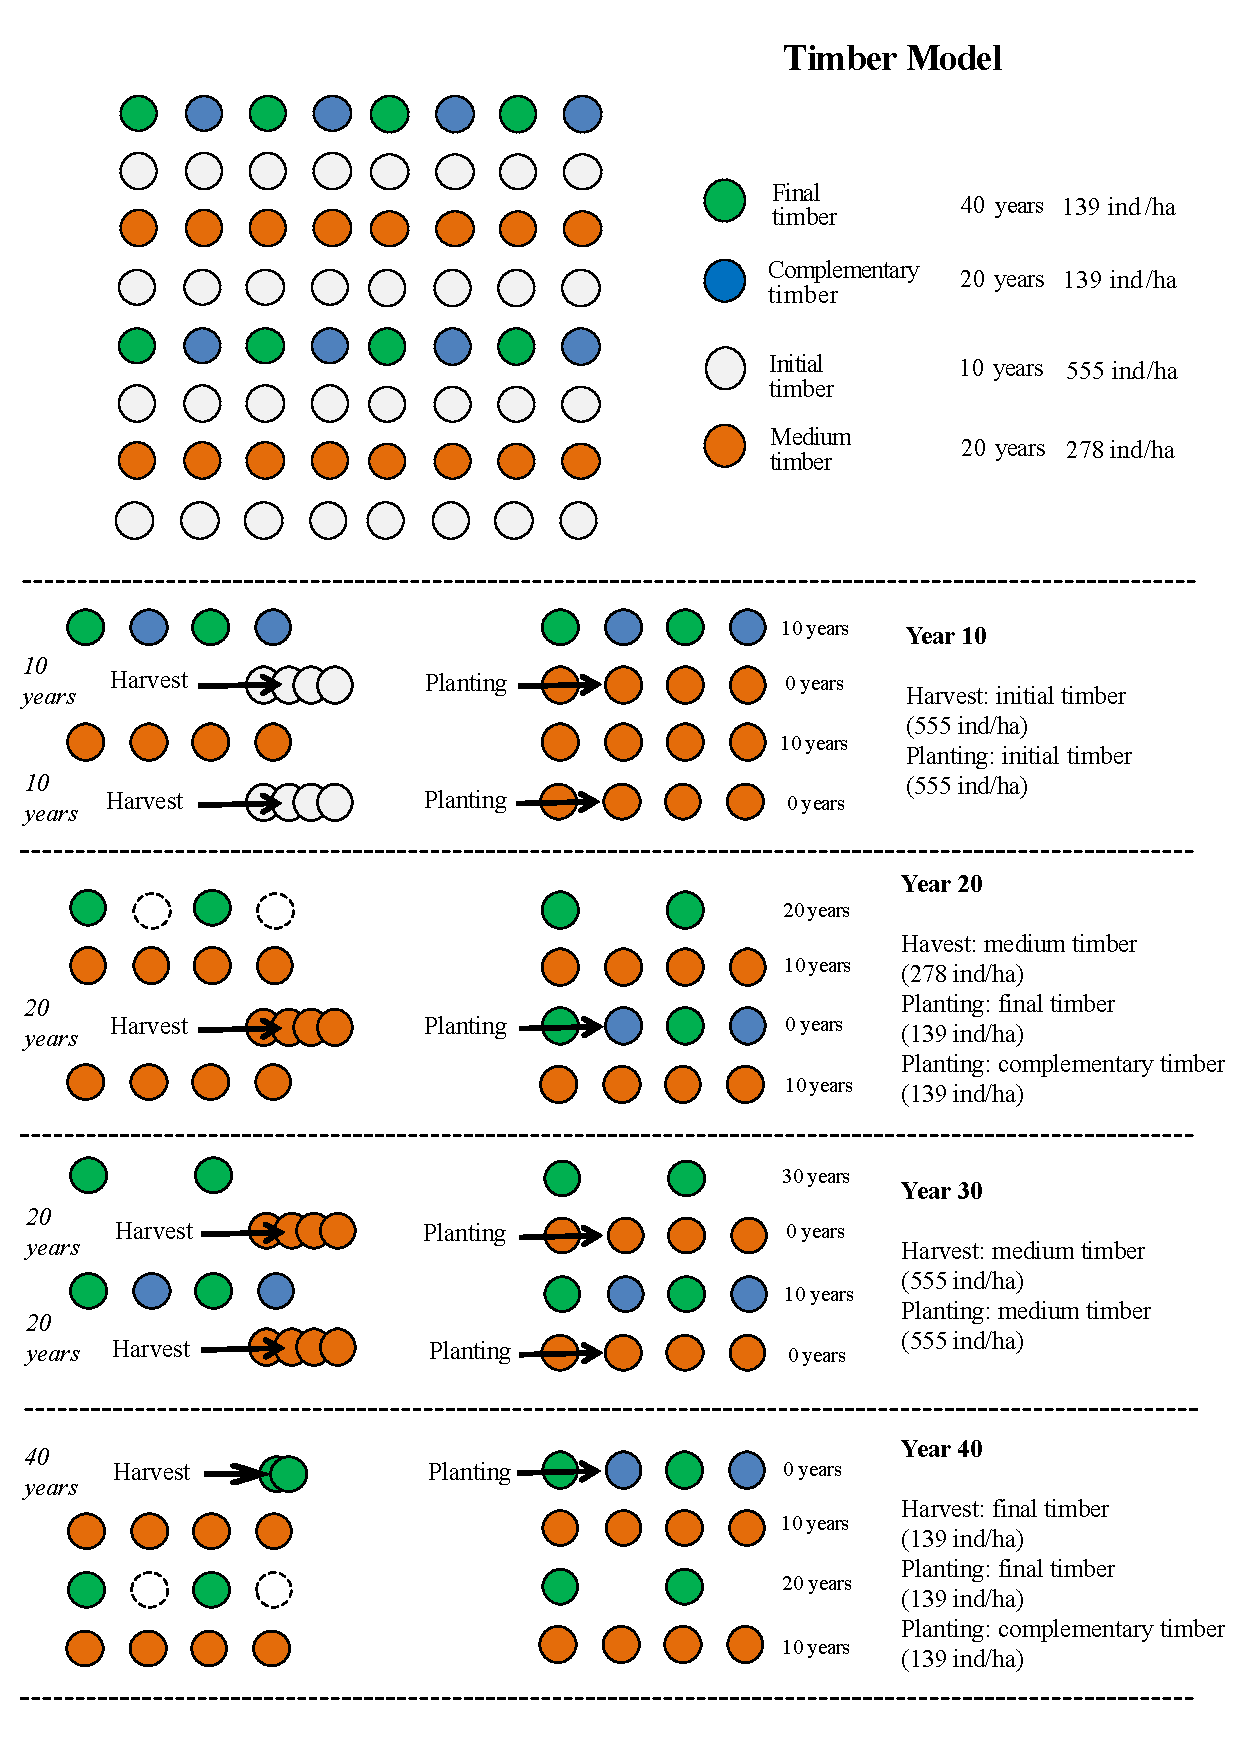
\includegraphics[width=\textwidth]{pictureve/socio-modelomadeira.pdf}
\caption{Economic exploitation model of Legal Reserve exclusively with timber species. }
\label{fig:modelmadeira}
\end{figure}

  \begin{figure}
\centering
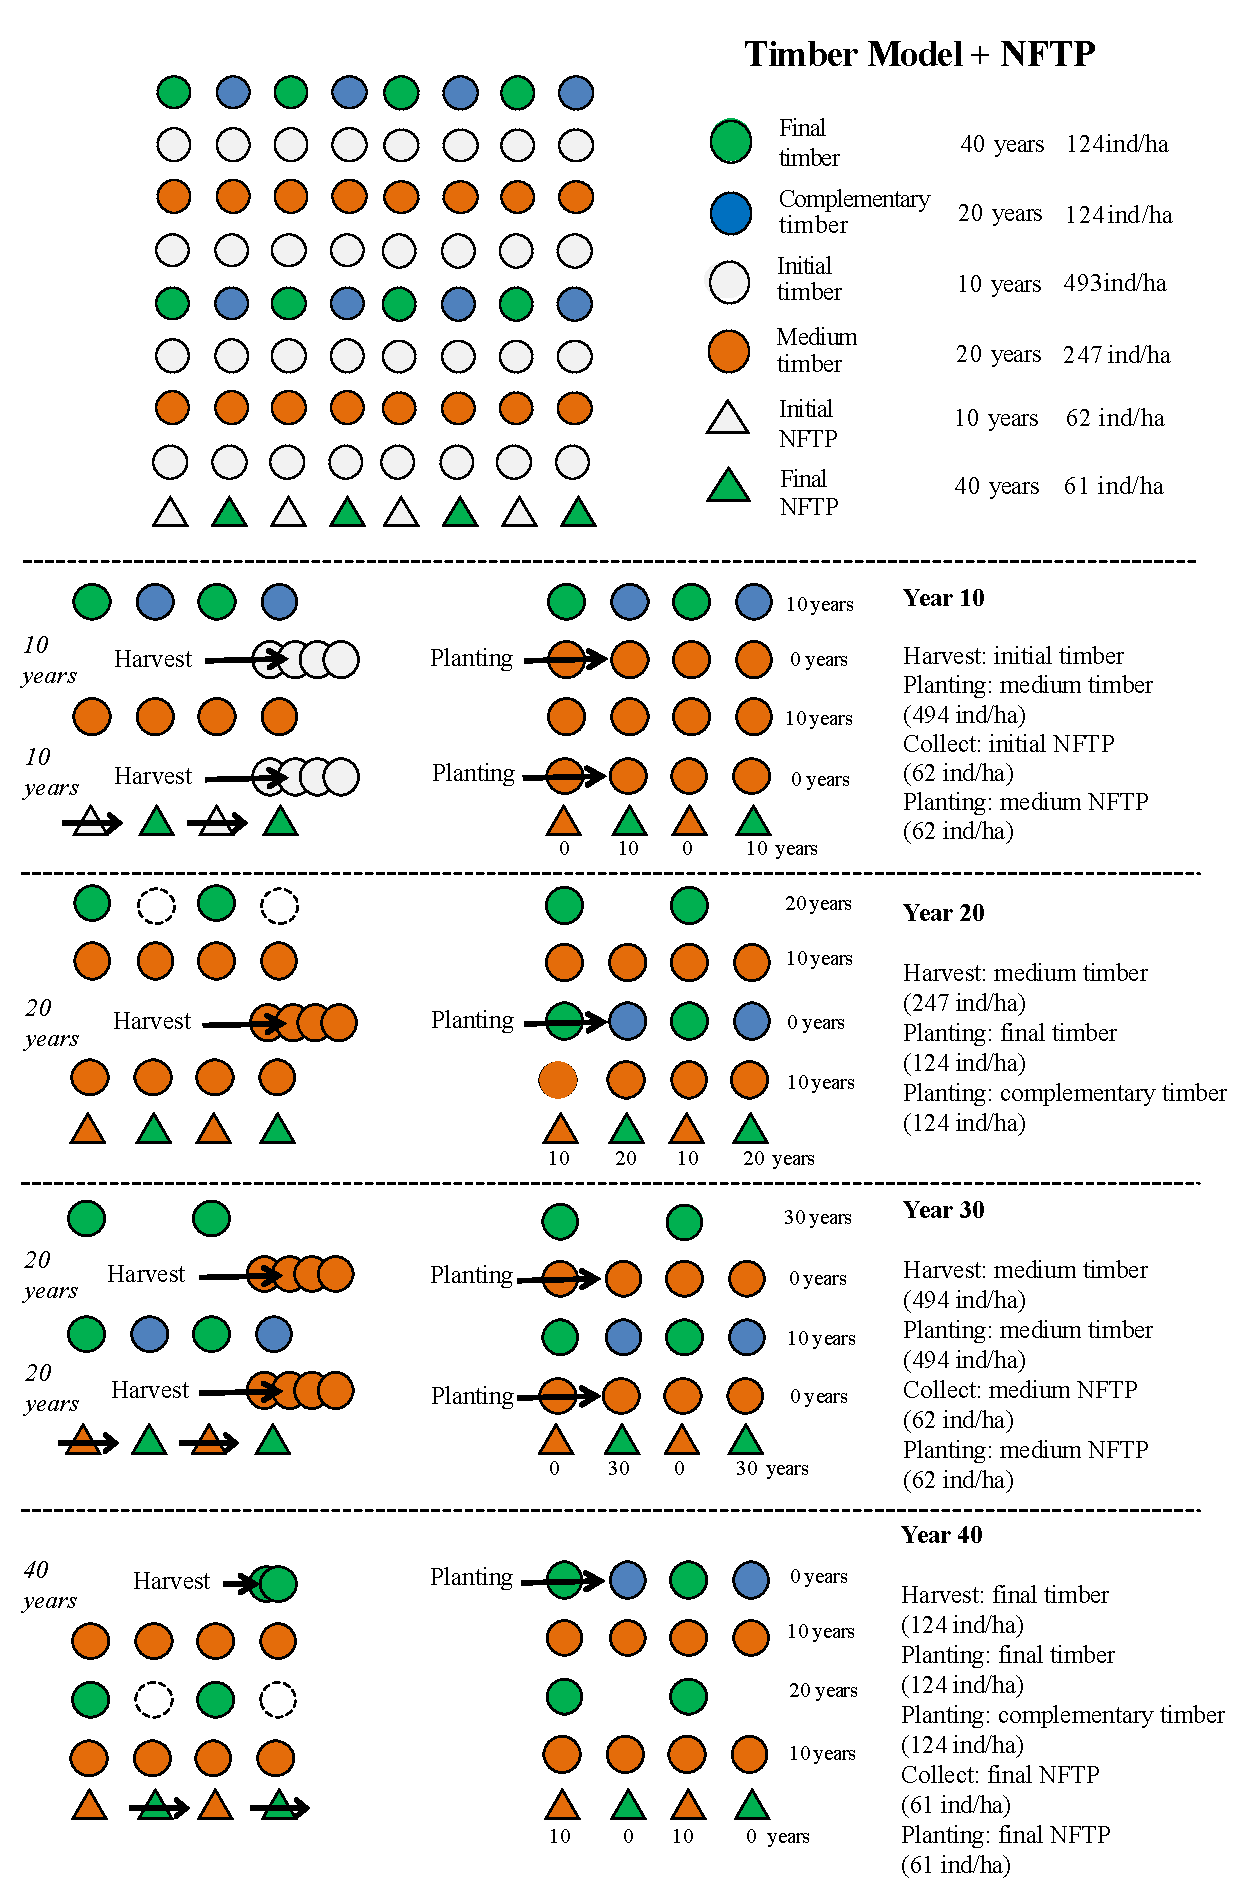
\includegraphics[width=\textwidth]{pictureve/socio-modeloNTFP.pdf}
\caption{Economic exploitation model of Legal Reserve with timber species and non timber forest products (NTFP).} \label{fig:modelNTFP}
\end{figure}

%----------------------------------------------------------------------------------------
%	CHAPTER 5: Overview of the FLR and Ecosytem services relation 
%----------------------------------------------------------------------------------------
%\chapterimage{SE.jpg} % Chapter heading image

%\input{Overview.tex}

%----------------------------------------------------------------------------------------
%	Preliminary Recommendations
%----------------------------------------------------------------------------------------
\chapterimage{recommend.png} % Chapter heading image




%----------------------------------------------------------------------------------------
%	CHAPTER: Recommendation
%----------------------------------------------------------------------------------------

\chapter{Preliminary Recommendations} \label{ch:recom}


Forest and landscape restoration aims to conserve biodiversity, safeguard essential ecosystem services for human well-being, and achieve social and economic benefits. Here, we recommend a series of best practices to guide decision makers, scientists and practitioners to achieve these goals and scale-up restoration. We identified these practices based on our results and on literature review focused on lessons learned and drivers for success of restoration initiatives. The ideal framework considers a transdisciplinary, participatory and adaptive management approach. 

The FLR mindset includes biophysical and socioeconomic aspects, as described on Table \ref{table:recommend}, and demands: (i) a better picture of social and environmental perceptions, (ii) multistakeholders involvement, (iii) socio-economic benefits evaluation and promotion, (iv) technical assistance, (v) spatial planning, (vi) attention to ecosystem services provision (as biodiversity conservation, carbon sequestration and water security), (vii) monitoring at multiple scales, (viii) communication and knowledge transfer. These practices can facilitate, stimulate and optimize restoration actions, reducing restoration costs and associated conflicts while optimizing its benefits.

\newpage

%%% to make table continues....
% \begin{table}
% \caption{A table}
% . . .
% \end{table}
% . . .
% \begin{table}\ContinuedFloat
% \caption{A table (cont.)}
% . . .
% \end{table}

{\small 
\begin{table} 
\caption{Main recommendations to achieve forest landscape restoration in Brazil.}
\begin{tabular}{|m{5.2cm}|m{5.5cm}|m{4.5cm}|}
\hline
\multicolumn{2}{|c|}{\bfseries Recommendation} & \bfseries Examples from literature    \\ 
\hline
\bfseries Restore with a landscape mindset      &Move beyond tree planting and incorporate both biophysical and socioeconomic aspects in the planning and implementation of restoration at the landscape level   &Dudley et al. 2002, Guariguata and Brancalion 2014, Brancalion et al. 2013, Mansurian et al. 2017     \\ 
\cline{1-3}
\multirow{2}{*}{\bfseries \makecell[l]{Capture and evaluate social and \\ environmental perceptions}}    &Understand the historical, cultural and economic backgrounds of each landscape and incorporate them at the outset of projects    &Ball et al. 2014,  Guariguata and Brancalion 2014 \\
\cline{2-3}   
&Evaluate the environmental perception and awareness of local communities   &Muler 2014, Lemgruber 2017  \\ 
\cline{1-3}
\multirow{2}{*}{\bfseries \makecell[l]{Foster bottom-up and \\ horizontal negociation \\ with stakholders}}  &Encourage local participation and involvement in restoration initiatives  &Le et al. 2012, Meli et al. 2017, Vieira et al. 2009, Ecker, 2016, Evans and Guariguata 2016 \\
\cline{2-3}  
& Integrate the aims and needs of different stakeholders   &Ball et al. 2014,  Guariguata and Brancalion 2014, Le et al. 2012, Brancalion et al. 2013, Meli et al. 2017 \\
\cline{2-3} 
& Promote space for negotiated decision-making  &Guariguata and Brancalion 2014, McGrath et al. 2008 \\
\cline{1-3}
\multirow{2}{*}{\bfseries \makecell[l]{Consider and promote socio-\\ economic benefits}}   &Promote integrated production systems (agroforestry, silvipasture, aquaculture)  &Le et al. 2012, Mansourian et al. 2014; Guariguata and Brancalion 2014, Jenkins at al. 2004, Menz et al. 2012, Meli et al. 2017, Veira et al. 2009, Ball et al. 2014  \\
\cline{2-3}
&Revise legal frameworks to broaden the possibilities for exploitation of native plant species  &Ball et al. 2014; Guariguata and  Brancalion 2014, Aronson 2010 \\
\cline{2-3}
&Promote marketing prospection of bidiversity products (timber and non-timber) and benefits from the restoration market chain     &Le et al. 2012, Jenkins et al. 2004, Ball and Brancalion 2016 \\
\cline{2-3}
&Encourage the creation of jobs in the restoration chain  &Calmon et al. 2011, ITPA 2010, IPEA 2015 \\
\cline{2-3}
&Encourage payment for ecosystem services polices   &Alves-Pinto et al. 2018, Grima et al. 2015, Zanella et al. 2014 \\
\cline{1-3}
\multirow{2}{*}{\bfseries Boost technical assistance}   &Improve rural extension and training  &Le et al. 2012, Pinto et al. 2014, Evans and Guariguata 2016  \\
\cline{2-3}
&Diversify restoration techniques according to local features  &Martins 2018  \\
\cline{2-3}
&Consider functional diversity when selecting species for planting  &Brancalion and Holl 2016  \\
\cline{2-3}
&Recognize natural regeneration as a relevant method for upscaling restoration  &Strassburg et al. 2016, Crouzeilles et al. 2017, Latawiec et al. 2016  \\
\hline
\end{tabular}





\label{table:recommend}
\end{table}
}
\newpage


{\small 
\begin{table} 
\ContinuedFloat 
\caption{Main recommendations to achieve forest landscape restoration in Brazil (Continued).}
%\label{table:recommend2}

% Continuação da tablerecommend
\begin{tabular}{|m{5.2cm}|m{5.5cm}|m{4.5cm}|}
\hline
\multicolumn{2}{|c|}{\bfseries Recommendation} & \bfseries Examples from literature    \\ 
\hline
\bfseries Boost technical assistance   &Promote rural innovations  &Pannell et al. 2006, Knight et al. 2010 \\
\cline{1-3}
\bfseries Consider spatial planning  &Prioritize FLR in areas with highest socio-ecological benefits per unit of cost  & Metzger et al. 2017, IIS 2017, Strassburg et al. 2018  \\
\cline{2-3}
&Identify scenarios focused on multiple outcomes  & Metzger et al. 2017, IIS 2017, Strassburg et al. 2018  \\ 
\cline{2-3}
&Consider the trade-offs and synergies among different restoration outcomes and targets to promote win-win solutions & Metzger et al. 2017, IIS 2017, Strassburg et al. 2018  \\ 
\cline{2-3}
&Incorporate climate changes projections into restoration planning, recognizing FLR as an ecosystem-based adaptation and mitigation to climate change  &Perry et al. 2015, Kane et al. 2017, Scarano and Ceotto 2015, Kasecker et al. 2017  \\
\cline{1-3}
\multirow{2}{*}{\bfseries \makecell[l]{Maximize biodiversity \\ conservation}}  &Increase landscape conectivity through stepping stones and corridors  &Crouzeilles et al. 2015, Rudnick et al. 2012, Tambosi et al. 2014, Watson et al. 2017  \\
\cline{2-3}
&Promote biodiversity-friendly land use systems to enhance matrix permeability to species dispersal, such as biodiverse rather than simplified agroforesty systems  &Watson et al. 2017, Donald and Evans 2006, Tambosi et al. 2014, Santos et al. 2018  \\
\cline{1-3}
\multirow{2}{*}{\bfseries Maximize carbon sequestration}  &Balance natural regeneration and active restoration to increase biomass accumulation over time  &Chazdon and Guariguata 2016, Crouzeilles et al. 2017  \\
\cline{2-3}
&Introduce species with greater rooting depth   &Stanturf et al. 2017  \\
\cline{2-3}
&Implement soil conservation measures to reduce erosion  &Stanturf et al. 2017  \\
\cline{2-3}
&Promote soil amendment to foster organic matter accumulation in the soil  &Stanturf et al. 2017  \\
\cline{1-3}
\multirow{2}{*}{\bfseries \makecell[l]{Maximize water quality \\ and provision}}  &Restore riparian and steepest slopes forests to prevent sediments from reaching the water bodies  &Saad et al. 2018  \\
\cline{2-3}
&Restore high altitude forests to improve water infiltration and reduce erosion, sedimentation, and downstream flooding  &Viviroli and Weingartner 2004, Bruijnzeel et al. 2011, Ghazoul and Sheil 2010, Ramírez et al. 2017  \\
\cline{2-3}
&Restore in areas where raises in rainfall are expected  &Ellison et al. 2017, Layton and Ellison 2016, Makarieva et al. 2006 \\
\hline 
\end{tabular}

\end{table}
} 

\newpage

{\small
\begin{table} 
\ContinuedFloat
\caption{Main recommendations to achieve forest landscape restoration in Brazil (Continued).}

%Continuacao (3) da Tabela recommend

\begin{tabular}{|m{5.2cm}|m{5.5cm}|m{4.5cm}|}
\hline
\multicolumn{2}{|c|}{\bfseries Recommendation} & \bfseries Examples from literature    \\ 
\hline
\multirow{2}{*}{\bfseries \makecell[l]{Implement long-term \\ monitoring at multiple scales}}  &Set specific targets, measurable goals, and objectives at the outset of projects  &Wortley et al. 2013  \\
\cline{2-3}
&Improve the application of time-series remote sensing monitoring on restoration projects  &Evans and Guariguata 2016  \\
\cline{2-3}
&Assess restoration quality and socioeconomic dimensions through on-the-ground monitoring over time  &FAO, CIFOR, IFRI \& World Bank 2016  \\
\cline{2-3}
&Encourage participatory monitoring   &Evans and Guariguata 2016, Ball and Brancalion 2016, Pinto et al. 2014, Meli et al.2017, Brancalion et al. 2013, Mansourian et al. 2017, McGrath et al. 2008  \\
\cline{1-3}
\multirow{2}{*}{\bfseries \makecell[l]{Foster communication and \\ knwoledge transfer}}   &Raise awareness of restoration benefits and limitations  &Terry et al. 2012, Brancalion et al. 2014 \\
\cline{2-3}
&Share knowledge in accessible communication frameworks  &Brancalion et al. 2013, Meli et al. 2017, Pinto et al. 2014, Evans and Guariguata 2016, Menz et al. 2013  \\
\cline{2-3}
&Promote knowledge exchange among stakeholders of different sectors and from different landscapes  &Terry et al. 2012, Brancalion et al. 2014  \\
\cline{2-3}
&Integrate educational and ecotourism activities in FLR iniciatives  &Muler 2014, Lemgruber 2017 \\
\hline 
\end{tabular}
%\label{table:recommend3}
\end{table}
}


% \section{Diretrizes para formuladores de políticas estaduais/federais}\label{sec:politcs}

% Well-preserved forests should be conserved and expanded, yet adopting more environmentally friendly land management practices in agricultural landscapes is a good complementary strategy. Policies focused on environmentally-friendly land management practices and FLR should advocate for the use of biodiverse agroforestry systems. The Native Vegetation Protection Law (N° 12.651/2012) allows the use of agroforestry systems to recover environmental debts in private rural properties, but do not recommend the type of agroforestry to be implemented. We recommend that biodiverse agroforestry should be favored over simple agroforestry systems as they can both provide higher values of biodiversity recovery (this report) and be more profitable (Miccolis et al. 2016).

% \section{Diretrizes para profissionais de restauracao}\label{sec:prof}

% We highlights the importance of incorporating landowners’ decision on forest restoration into spatial prioritization, but considering the ecological processes that occurs at the landscape scale, such as landscape connectivity. 


%----------------------------------------------------------------------------------------
%	BIBLIOGRAPHY
%----------------------------------------------------------------------------------------

\chapterimage{referencias.png} % Chapter heading image

\bibliographystyle{unsrt}
\bibliography{IKI}


\end{document}
